\documentclass[times, 10pt]{thesisMDH}



%Package importation 
\usepackage[ddmmyyyy]{datetime}
\usepackage[pdfborder={0 0 0},colorlinks=true,urlcolor=blue,citecolor=red,bookmarks=false]{hyperref}
\usepackage{graphicx}
\usepackage{subcaption}
\usepackage{caption}

%reference package
\usepackage{hyperref}
\usepackage{pdfpages}


%Figure & table config
\usepackage{booktabs} % For professional lines
\usepackage{tabularx} % For auto-wrapping text
\usepackage{xcolor}




\addbibresource{references.bib}

\fancyHeader{Maven-01}{Vinh Thanh Nguyen }

\university{University of Science and Technologies Hanoi}

\department{Information Communication and Technologies department}

\subject{Thesis for the Degree of Master of Science in Data Science \& Robotics  }
\thesisTitle{Maven-01: A Teleopeated Rover Platform for Planetary Exploration }
\authorOne{Vinh Thanh Nguyen}{vinhnt.23bi14453@usth.edu.vn}

\supervisors{Pham Xuan Tung}{University of Science of Technologies Hanoi}


\theDate{\today} 

\begin{document}
\titlePage
% Begin actual text
\frontmatter

%========= Tables ==========
{\hypersetup{linkcolor=black}\tableofcontents}
\clearpage
{\hypersetup{linkcolor=black}\listoffigures}
\clearpage
{\hypersetup{linkcolor=black}\listoftables}


% Abstract 
% ============================= Abstract ==============================
\begin{abstract}
 This abstract summarizes the design, development, and functional improvements of MAVEN-01, a rover platform whose primary objective is to provide a highly customizable mobile system for research and educational purpose. The report elaborates on the rover’s design and the techniques used in its development, such as 3D printing.
Furthermore, in addition to the mechanical frame design, this paper also focuses on the electrical system implemented in the rover. Due to limited budget and time constraints, we selected the popular ESP32 microcontroller, which features built-in Wi-Fi and Bluetooth capabilities for teleoperation purposes. Other components were also carefully chosen to balance performance and cost. For example, the DHT11 or DHT12 sensors are suitable for temperature and humidity measurement, while the HC-SR04 sensor is used for distance measurement.
The paper also discusses practical challenges, including durability, reliability, and ease of maintenance.


\end{abstract}

\section{System Requirement \& Testing}

\subsection{Mechanical Design \& Mobility Requirement}
MAVEN-01 need to be a modular budget friendly 3D printed rover platform for research and educational 
purpose, easy to maintain.

For mobility, the rover was design to run on flat terrain and power efficient with 2 engine chassis version.
With 4 motors version, we expect MAVEN-01 has better off-road ability than the 2x4 version.

\subsubsection{Detailed Testing plan}

\begin{itemize}
    \item Terrain types: Road, glass, off road
    \item Obstacles height: 3cm \& 5cm 
\end{itemize}

\subsection{Electrical \& Power Requirement }
MAVEN-01 was design to have 3 power sources for each modular section like: control board, censors, mobility motors
for power efficient and easy maintenance. 

\subsubsection{Detailed testing plan}
\begin{itemize}
    \item Operation time: 2 hours
    \item Testing swappable battery 
\end{itemize}

\subsection{Software \& Control Requirement Testing}
\begin{itemize}
    \item Verify sensors data with other source: forecast, weather cast  
    \item Control latency < 5ms
    \item Testing the wifi connection cast from control board 
\end{itemize}




\newpage

\mainmatter
% ===== Content: Modify the structure according to your needs =======
\section{Introduction}
\label{sec:intro}

Alongside exploration tasks, the importance of developing teleoperated mobile systems has been recognized for a long time. Historically, humans have conducted exploration missions themselves, which remains effective for many low-risk and specific tasks. 
However, for higher-risk and more hazardous missions—such as volcanic surveys or planetary exploration—researchers rely on specialized vehicles known as \textit{rovers}.
For example, \href{https://www.nasa.gov/}{NASA} launched the \href{https://science.nasa.gov/mission/mer-opportunity/}{Opportunity} in 2003 and the \href{https://science.nasa.gov/mission/msl-curiosity/}{Curiosity} in 2012, two of the longest-operating missions on Mars, aimed at determining whether the planet could have supported life.

\par
Although each rover was designed for different specific missions and utilized distinct technologies, 
they share several common structural features. Both systems were designed to be controlled and monitored 
from NASA headquarters on Earth. Additionally, they were engineered for high reliability and strong terrain 
adaptability—key factors that serve as motivation for the development of our own rover platform.


\begin{figure}[h]
    \centering
    \begin{subfigure}{0.45\textwidth}
        \centering
        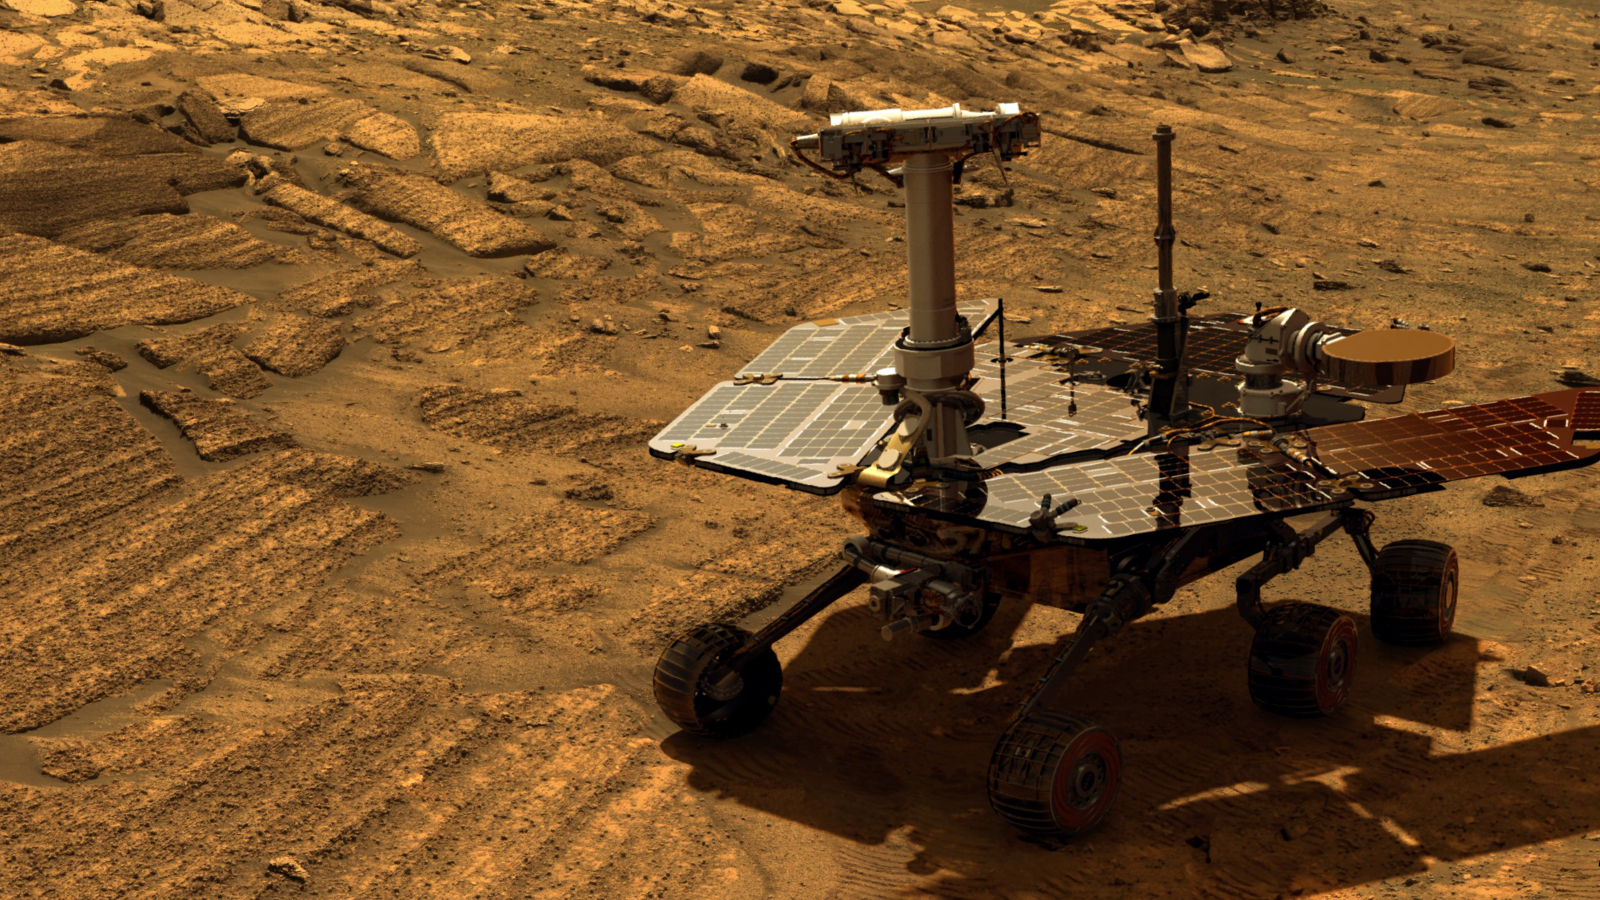
\includegraphics[width=\linewidth]{images/rover_reference /opportunity.jpg}
        \caption{Opportunity Rover}
        \label{fig:opportunity}
    \end{subfigure}
    \hfill
    \begin{subfigure}{0.45\textwidth}
        \centering
        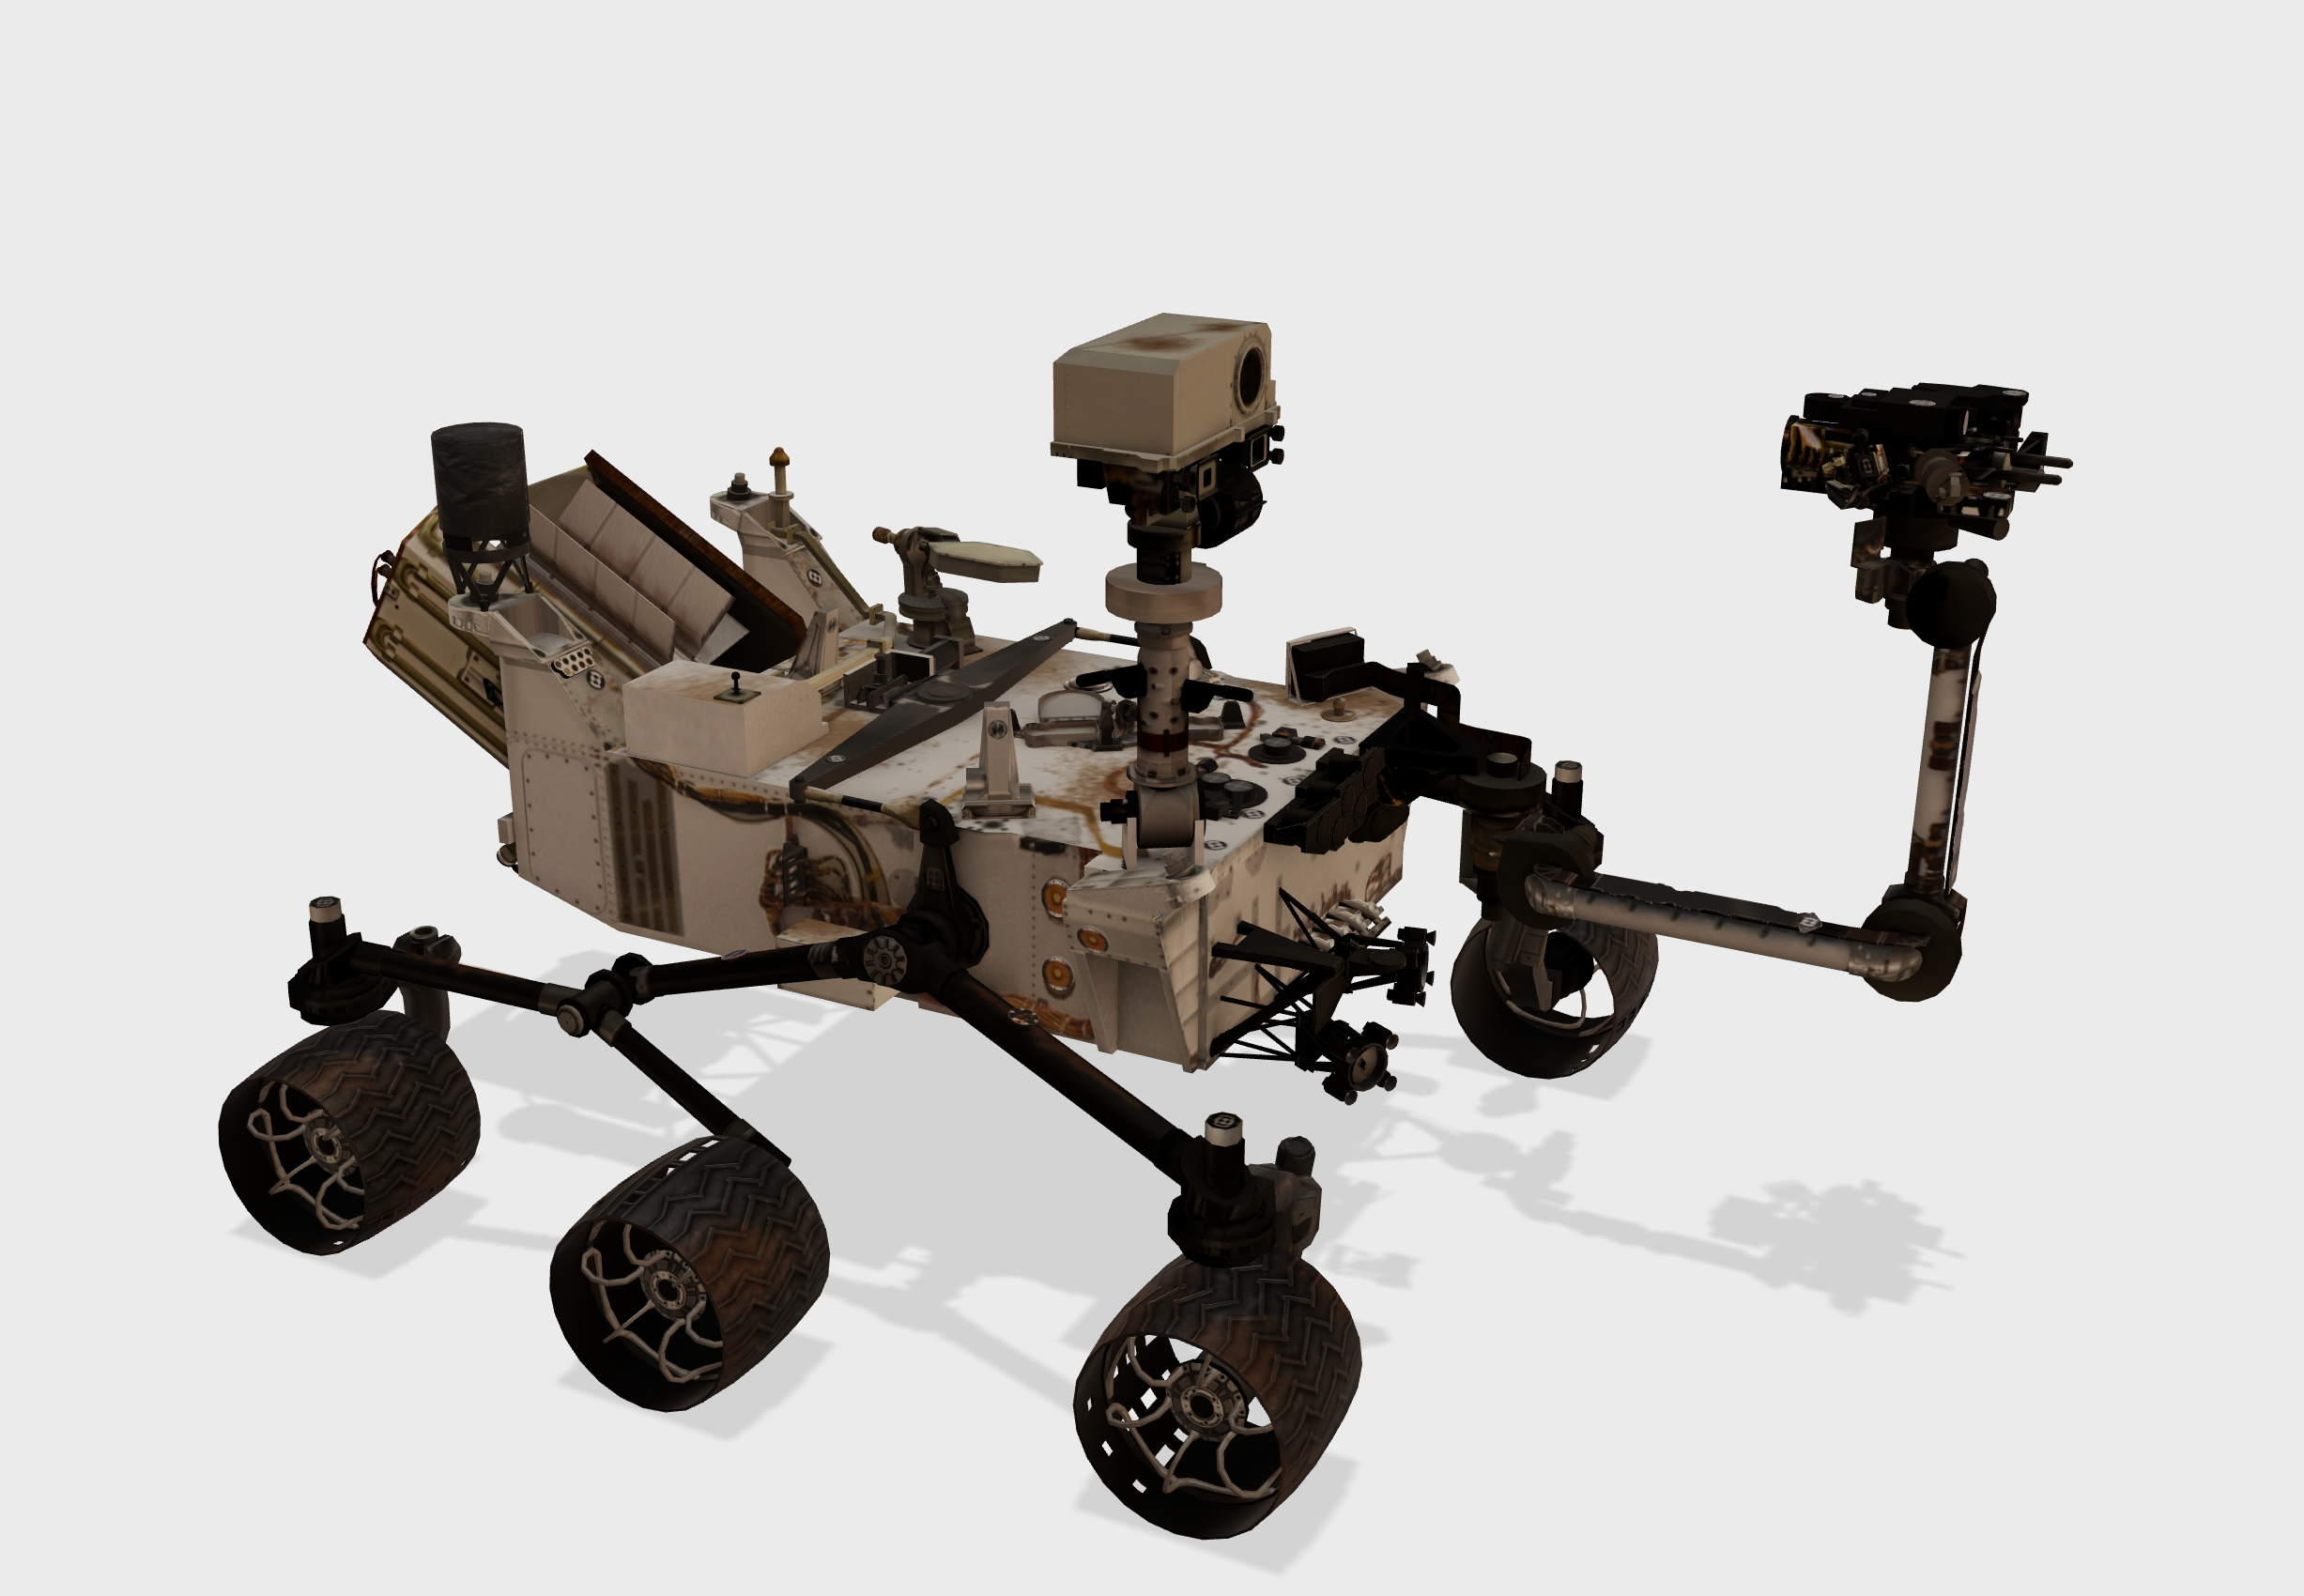
\includegraphics[width=\linewidth]{images/rover_reference /curiosity.png}
        \caption{Curiosity Rover}
        \label{fig:curiosity}
    \end{subfigure}
    
    \caption{Curiosity and Opportunity Rovers hold record for two longest operating time, 
    14 years (~5100 Sols) for Opportunity and 13.7 years (4863 Sols) for Curiosity.}
    \label{fig:rovers}
\end{figure}


This section introduces our rover platform, MAVEN-01, which represents the first iteration of our design. 
We are currently continuing its development to improve performance, durability, and reliability. 
Through multiple prototypes and design iterations—including unsuccessful attempts—MAVEN-01 has evolved with a clear objective: 
to provide a low-cost rover platform for research and experimental purposes using 3D printing technology.
The rover is designed to support customization for specific tasks, featuring multiple mounting holes 
on the top surface to accommodate additional components and modules.






\section{Mechanical Design}
\label{sec:background}

\subsection{Structure Design Overview}

\subsubsection{First version}
\par

MAVEN-01 was first designed as a two-tracked, tank-type vehicle platform using two 6V TT gear motors for each track. 
The size of the rover frame platform is 16.8 × 11 cm. The reason why the first body was small is due to the space limitation 
of the printing plate area of the Bambu Lab A1 Mini, which is our 3D printer. During the process, there were two material options: PLA and PETG. 
PETG is cheaper than PLA and offers higher durability and better heat resistance, but it is harder to print and requires careful storage 
due to its humidity-sensitive properties.

\vspace{1.5 em}
\par
We chose PLA for its easier printing process and better print consistency, which is more suitable for rapid prototyping and iterative design. 
PETG might be chosen for more specific missions that require higher durability in harsher environments.

\begin{figure}[H]
    \centering
    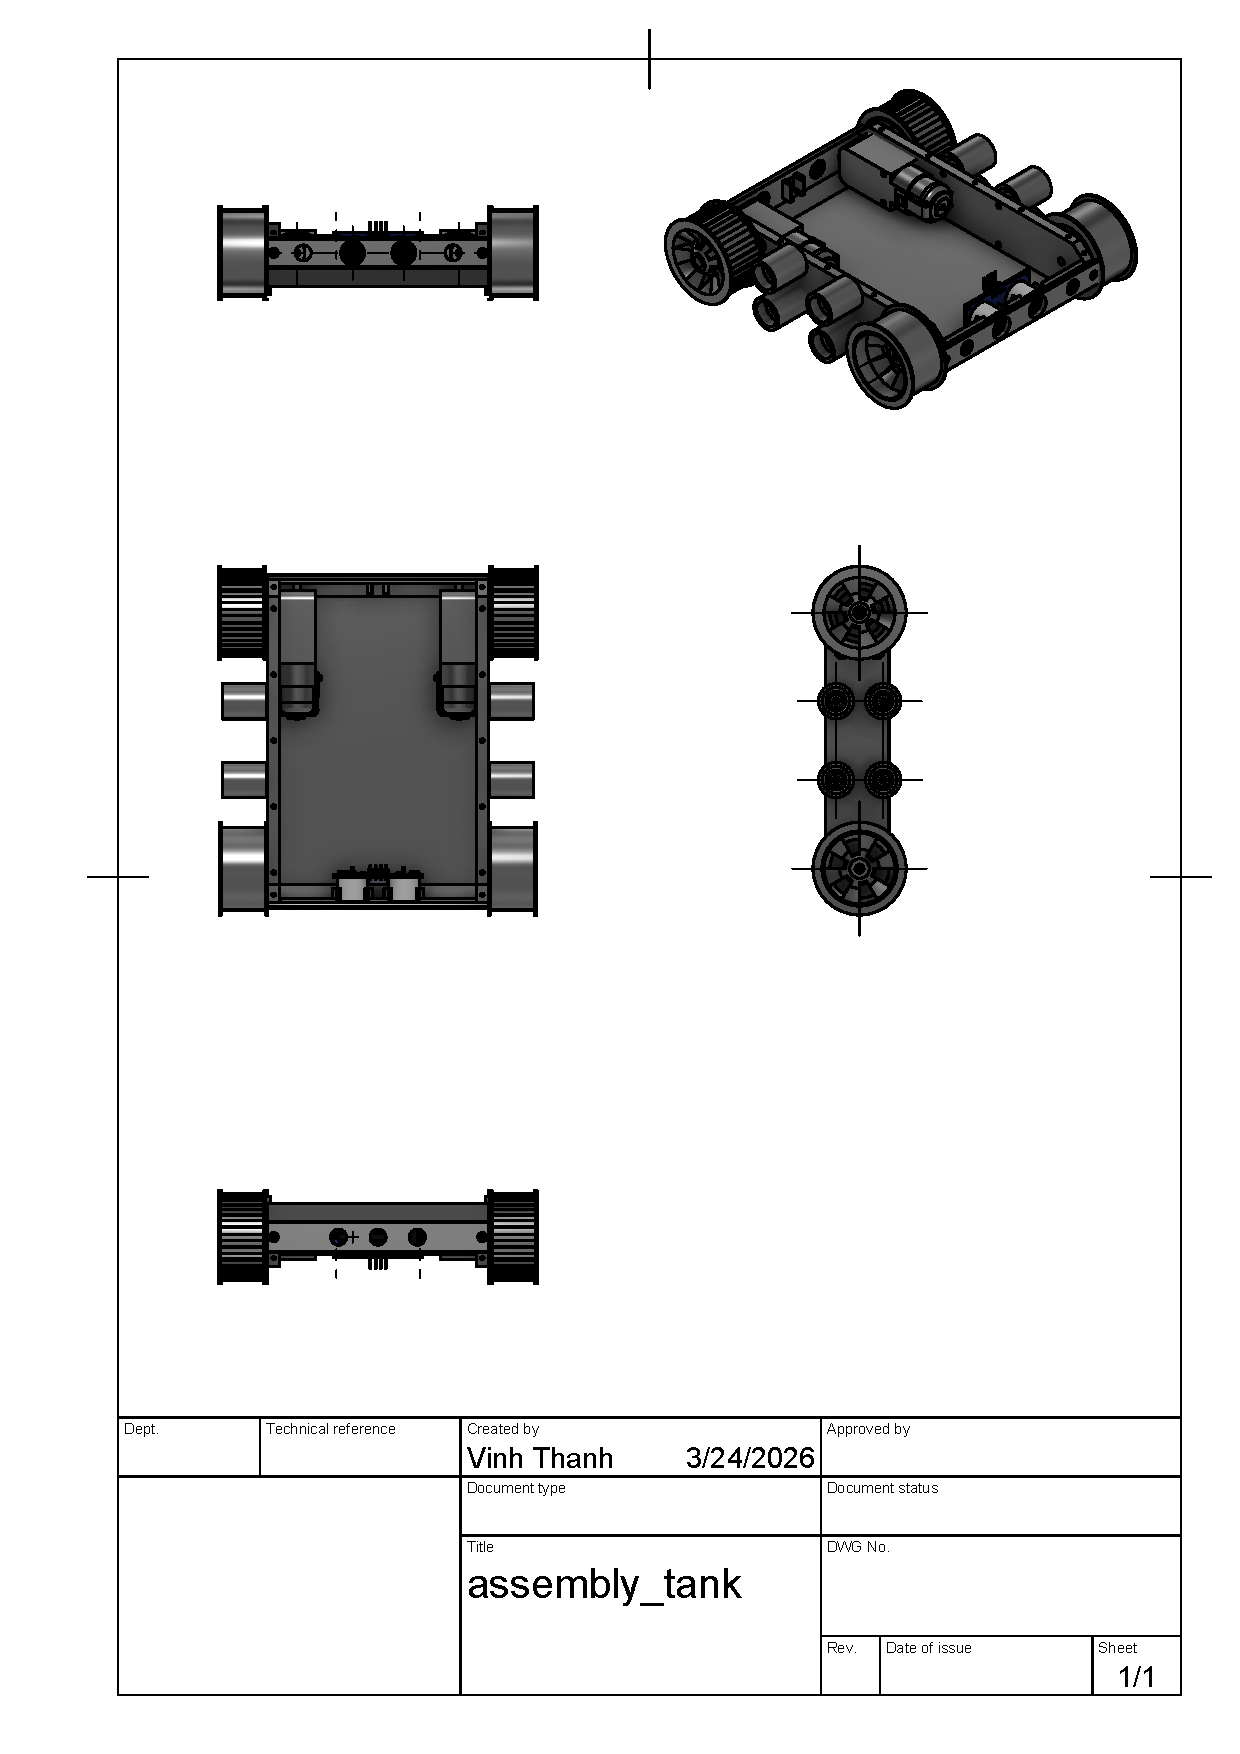
\includegraphics[width=0.75\linewidth]{images/blueprint/maven_01_first_prototype.pdf}
    \caption{Blueprint of MAVEN-01 first prototype}
    \label{fig:first_vers_blueprint}
\end{figure}


\text{Disadvantages}
However, there are some disadvantages in the first design that should be carefully considered. 
Due to the low ground clearance, this design cannot operate effectively in rugged terrain.

Another disadvantage is that the track can slip off the wheels due to the unstable drive wheel. 
In the first design, M4×30 screws and nuts are used to mount the drive wheel and front wheel. 
This design has a weakness: during testing, the screws wore into the wheel holes on the body, 
which caused the drive wheels to loosen over time, making the track structure weaker.

\vspace{1em}
The last weakness of this design is two engines are mounted inside the rover body, which 
occupy a large space, we can put more components inside base body. During operation time, two DC motor 
can generate heat which can effect on micro-control board, also not ideal for PLA body due to not limited heat resistance.


\begin{table}[h]
\centering
\begin{tabular}{|l|c|c|}
\hline
\textbf{Feature} & \textbf{PLA} & \textbf{PETG} \\
\hline
Printability & Very easy & Moderate \\
\hline
Strength & Strong but brittle & Strong and flexible \\
\hline
Temp. Resistance & Low ($\sim$70$^\circ$C) & Moderate ($\sim$85$^\circ$C) \\
\hline
Durability & Low outdoor durability & High UV resistance \\
\hline
Post-Processing & Easy to sand/paint & Harder to sand \\
\hline
\end{tabular}
\caption{Comparison of PLA and PETG specifications}
\label{tab:pla_vs_petg}
\end{table}

\subsubsection{Second Version}

\begin{figure}[H]
    \centering
    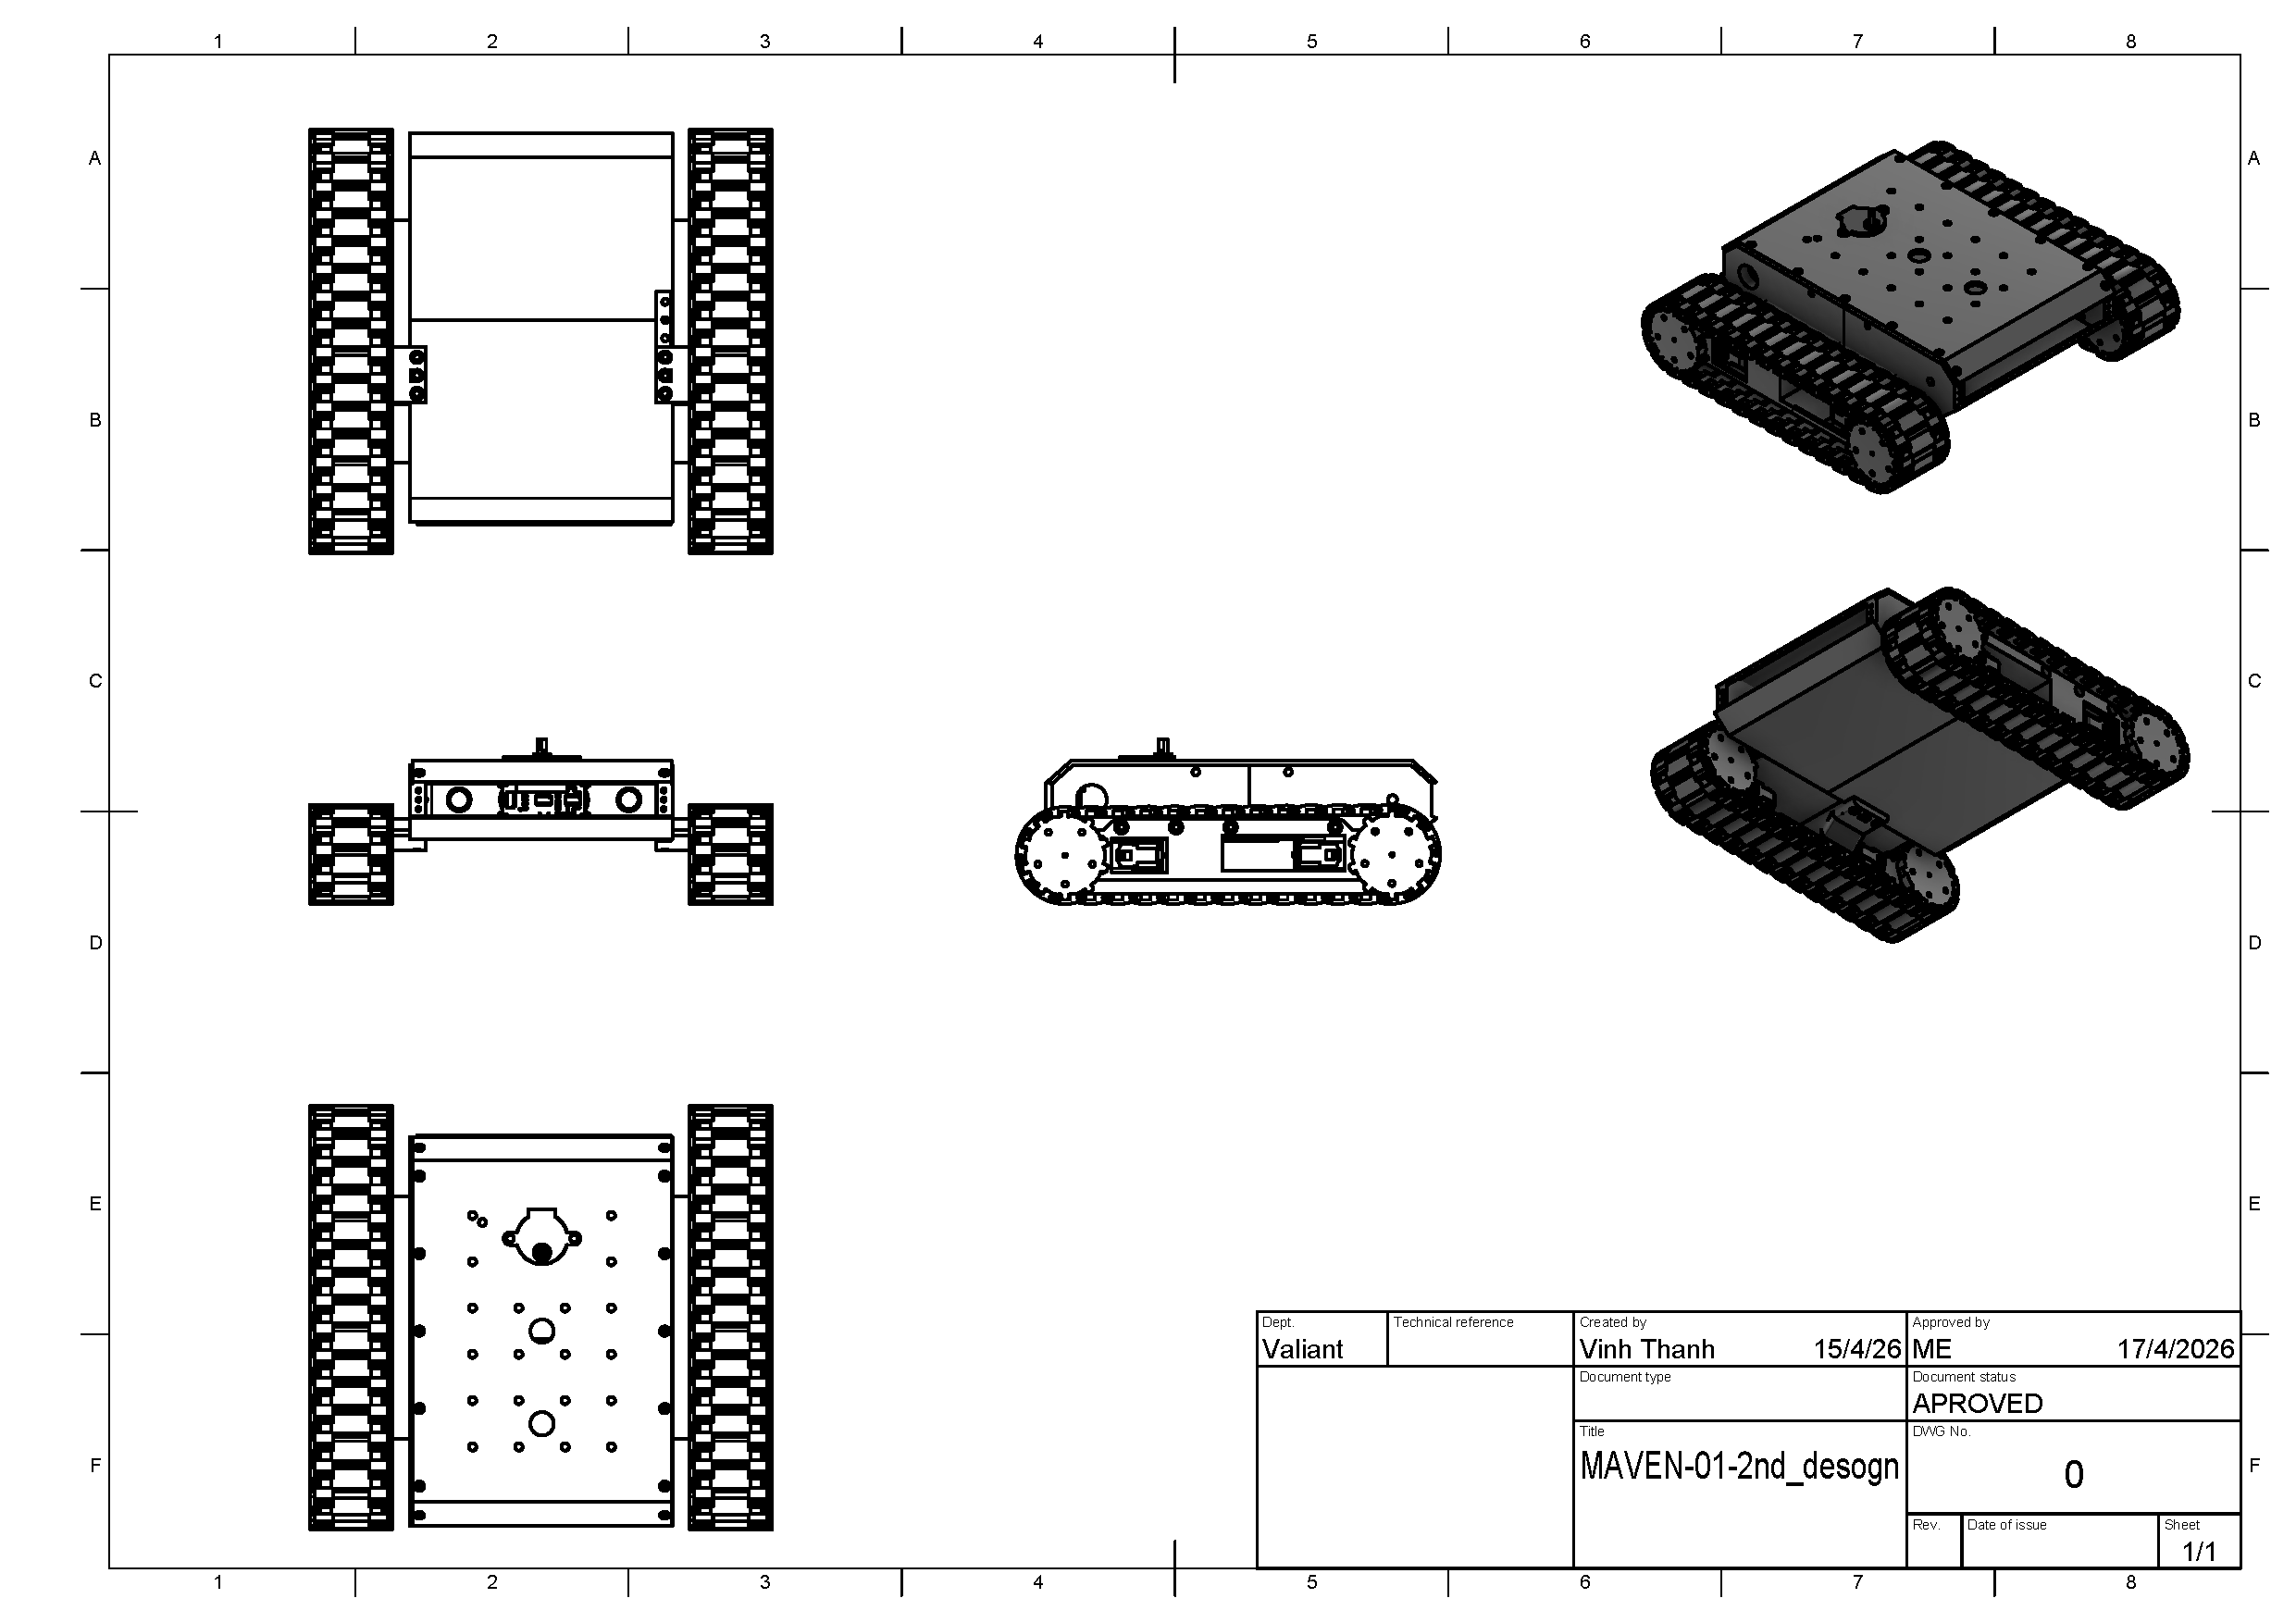
\includegraphics[width=0.95\linewidth]{images/blueprint/Maven-01-2nd-design.pdf}
    \caption{MAVEN-01 second prototype design using separate chassis with chained tracks (Single motor chassis) }
    \label{fig:chasis_1_engine_blueprint}
\end{figure}

\par
In this version, we improve the design  completely to fix the disadvantages of the first design. We move the track system into a separate module,
which allows more space in the base rover body. With the separate track module, the ground clearance can be higher, allowing MAVEN-01 to adapt to different terrain types and rough surfaces.
The \href{https://www.st.com/resource/en/datasheet/l298.pdf}{L298N} motor driver module and gear motor heating problems are also solved by the open-surface chassis design, which allows open-air ventilation to work as a cooling system.
My design inspired by \cite{TankTrack2024} but with some modified for better upgrade in the future.


\subsubsection{Chassis design}
\begin{figure}[H]
    \centering
    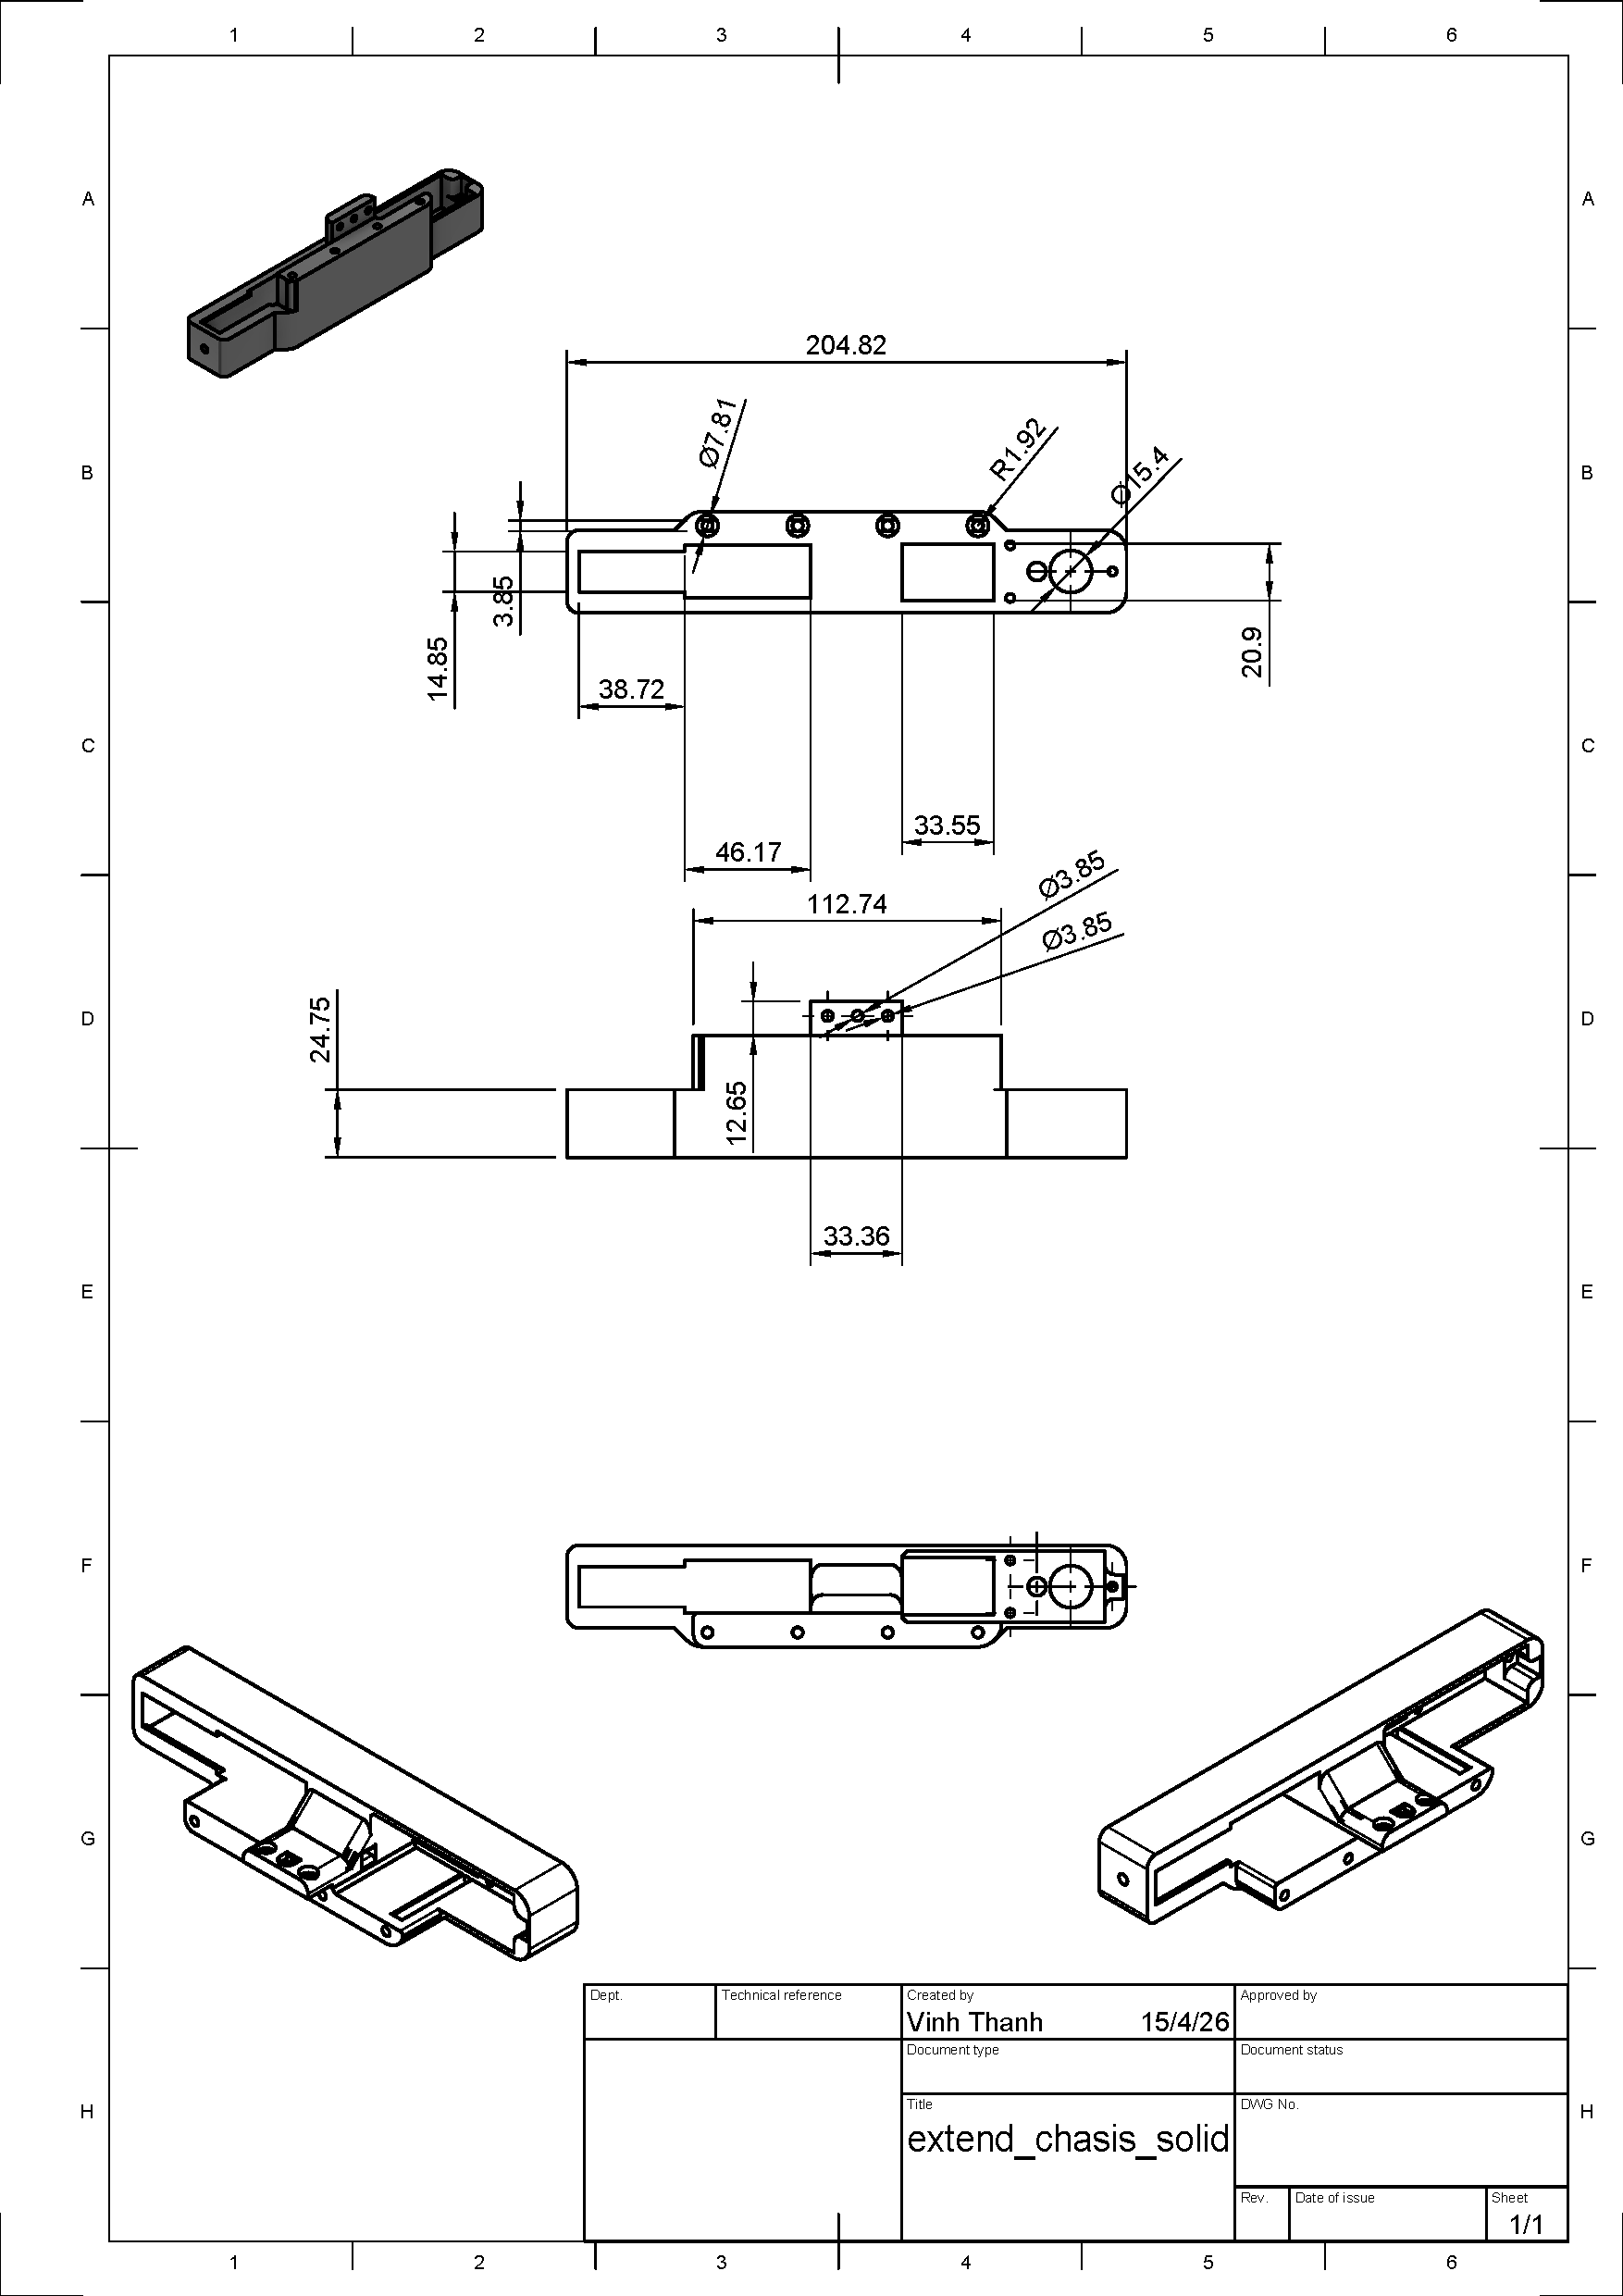
\includegraphics[width=0.9\linewidth]{images/blueprint/chassis_1_engine.pdf}
    \caption{Single motor chassis blueprint for 6V TT gear motor with open surface for motor air cooling }
    \label{fig:chasis_1_engine_blueprint}
\end{figure}

\vspace{2em}
\subsubsection{Drive wheel design}

\begin{figure}[H]
    \centering
    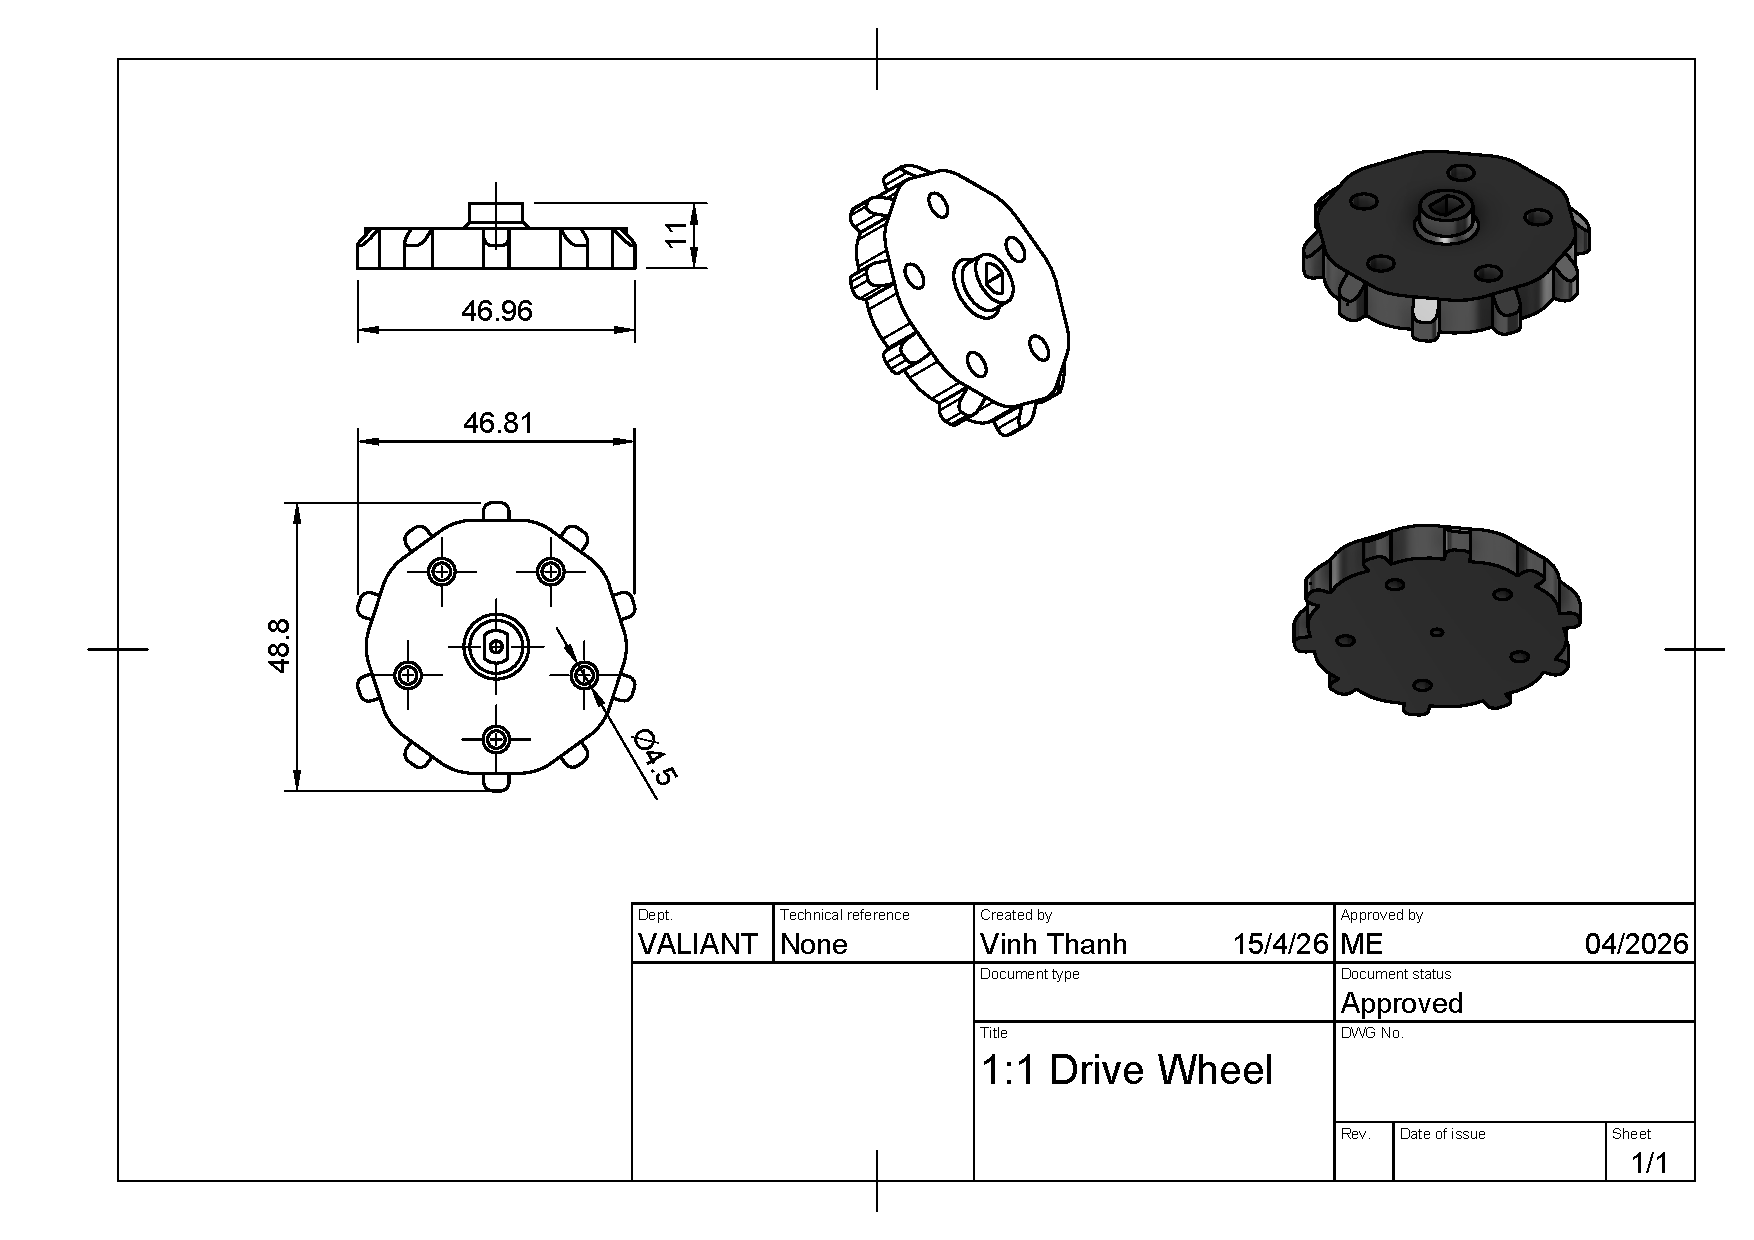
\includegraphics[width=0.8\linewidth]{images/blueprint/drive_wheels.pdf}
    \caption{Driver wheels blueprint for MAVEN-01}
    \label{fig:drive_wheels_blueprint}
\end{figure}

Each TT motor will have two drive wheels act as anchors for track chains attached. Drive wheels can be 
attached info motor axises using glue or M2x10 to M2x12 tap screws. 

\vspace{1em}

\subsubsection{Passive wheel design}
\par
Passive wheel were design to attach 6700zz bearing for smooth rotation, 6700zz has size of 
15x10x4MM, mounted and screwed with M5x10 tap screw and M5 nuts as holding reinforcement. 
\par
\begin{figure}[H]
    \centering
    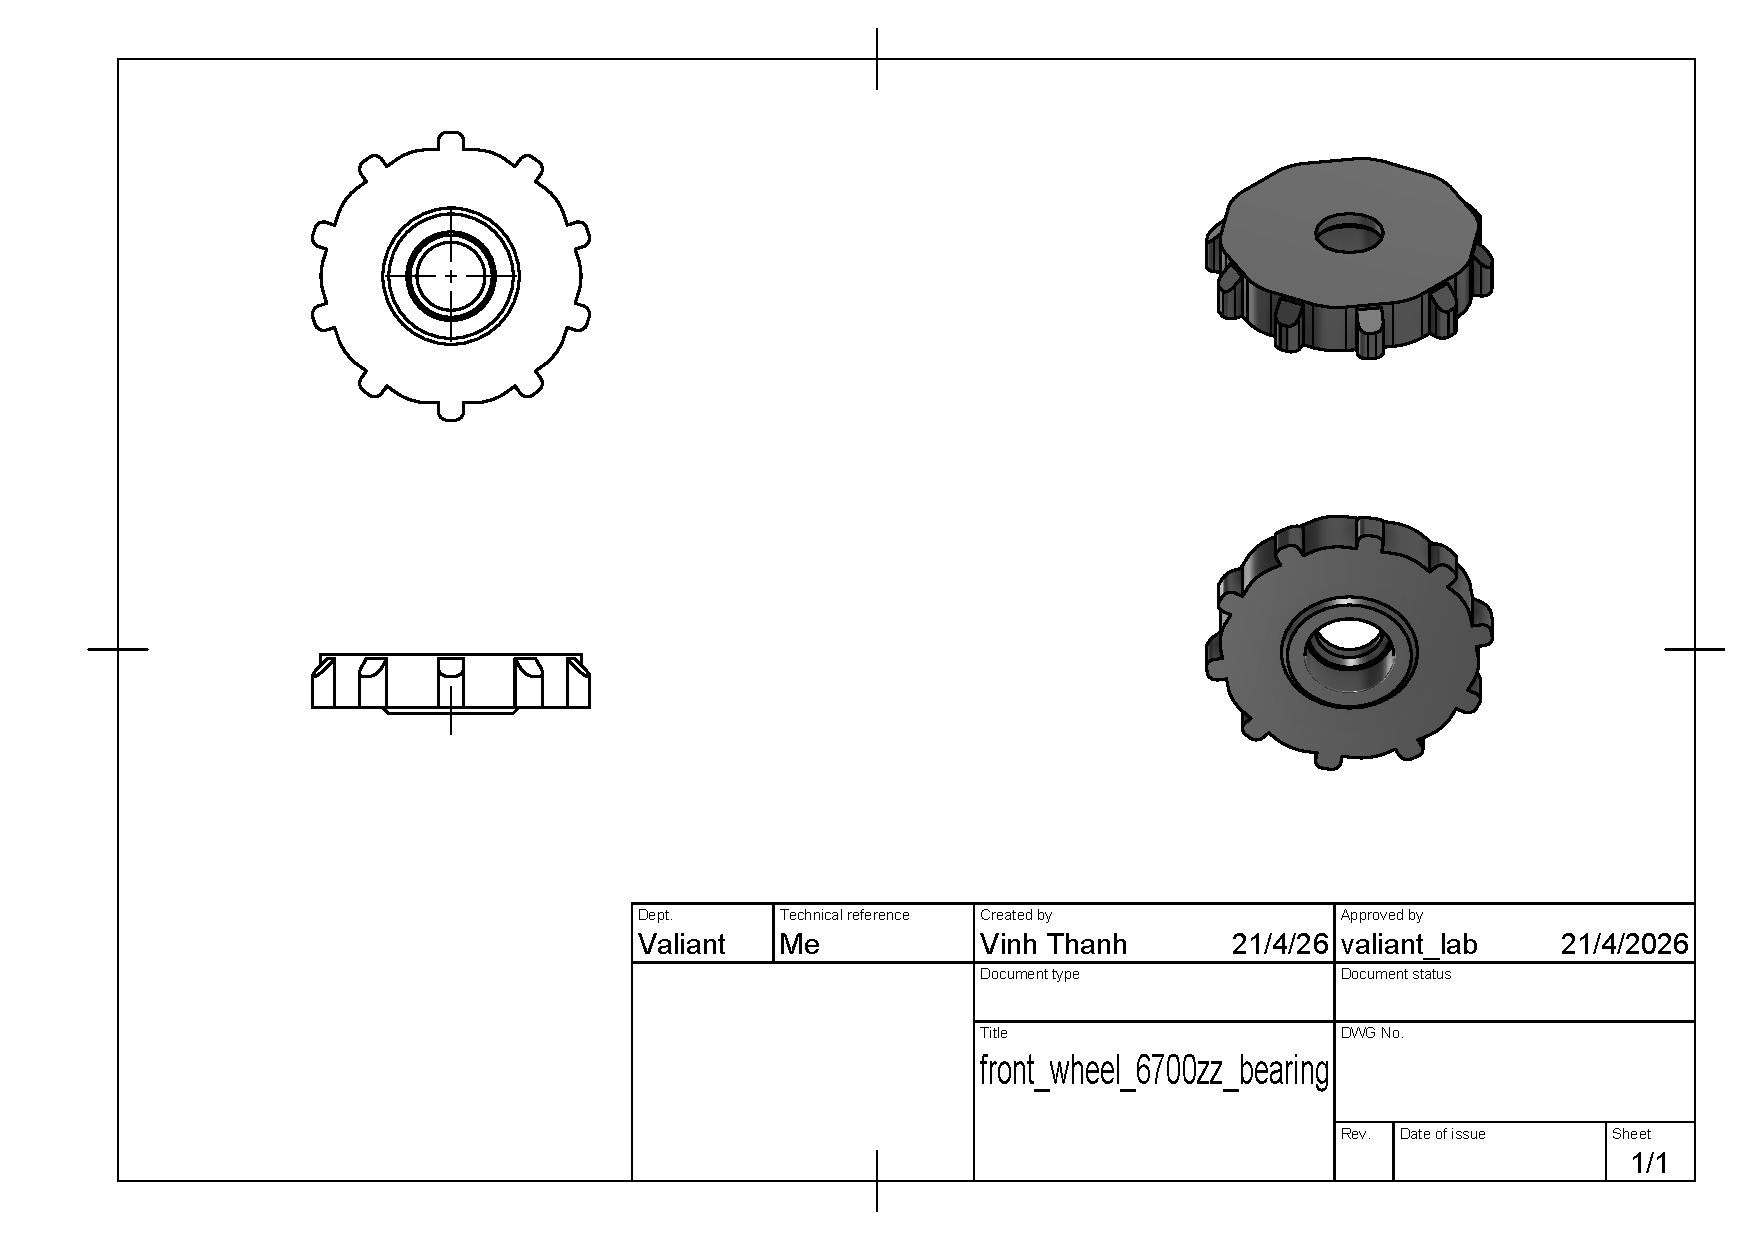
\includegraphics[width=0.80\linewidth]{images/blueprint/front_wheel_6700zz_bearing_oriented.pdf}
    \caption{Front wheels with 6700zz bearingblueprint for MAVEN-01}
    \label{fig:frontwheel_6700zz}
\end{figure}\vspace{1em}


\subsubsection{Front axis}
\vspace{1.5em}

\begin{figure}[H]
    \centering
    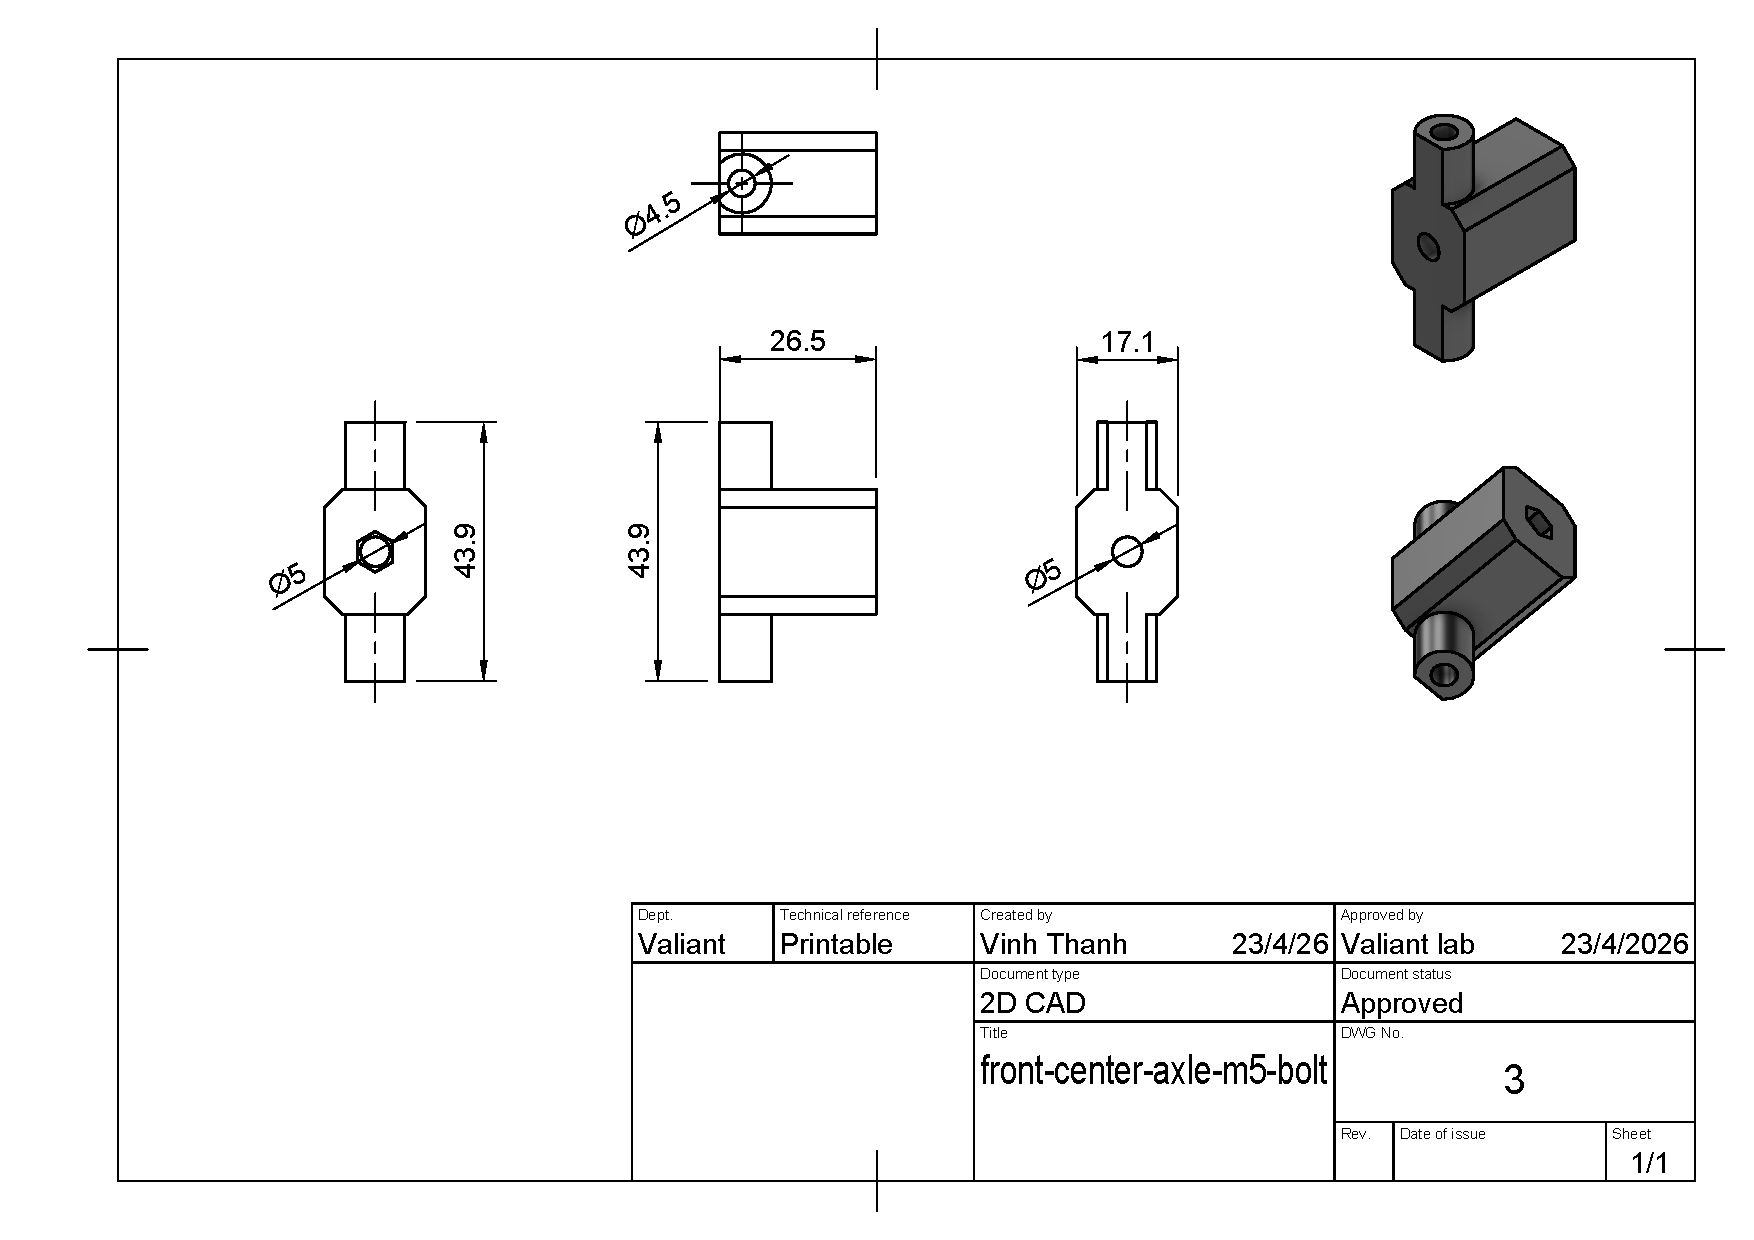
\includegraphics[width=0.78\linewidth]{images/blueprint/front-center-axle-m5-bolt_drawing.pdf}
    \caption{Front axis for front wheels for M5 bolts}
    \label{fig:frontwheel_axis_m5_bolt}
\end{figure}\vspace{1em}

\par
Front wheels of Maven-01 are designed not to be attached directly to the chassis;
they will be attached to a front wheel axis. The reason for separating this part from the chassis is that the front wheels are passive, 
which over time can be abraded. With the front wheels attached to the front axis instead of the chassis, 
they can be easily changed when worn out,and chassis replacement will not be required.


\subsubsection{Track chain}
\begin{figure}[H]
    \centering
    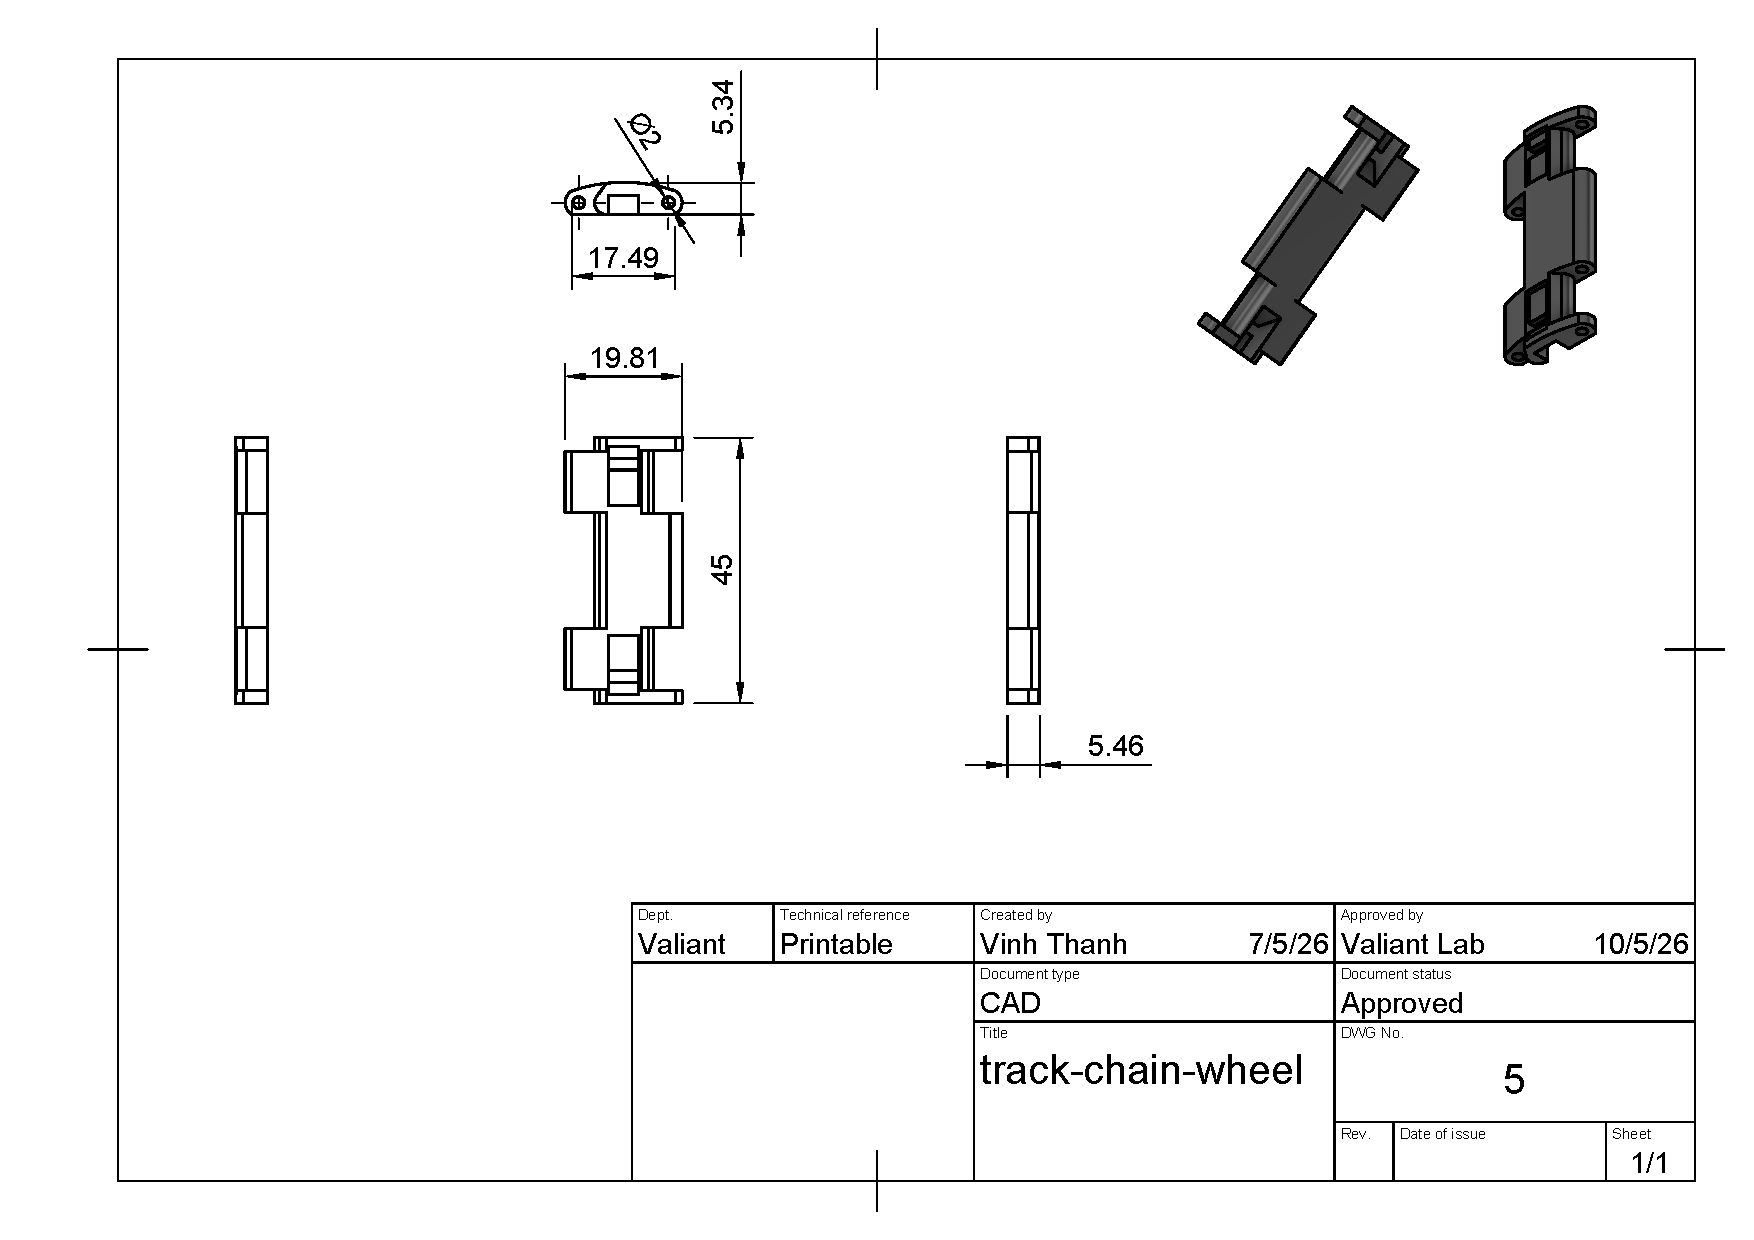
\includegraphics[width=0.75\linewidth]{images/blueprint/track_chain.pdf}
    \caption{Front axis for front wheels for M5 bolts}
    \label{fig:track_chain_blueprint}
\end{figure}\vspace{1em}
\par
MAVEN-01 uses an assembled chain design. In the first design, it used a rubber chain, 
but the wobbling axles caused the rubber track to become unstable, which could lead to 
derailment because there were no stable anchor points for the chain to mount onto both the 
front wheels and the drive wheels, which solved by this second design.

 %Structure design 
\newpage
\section{Electrical Design}
MAVEN-01 is designed to be an affordable autonomous vehicle platform for research and educational purposes, so
as we chose low range price electrical components but still make sure the rover has solid performance by price.

\vspace{1em}
\text{Power source}
We use two 6C 18650 lithium batteries as the main power source for most of the system, include motor, sensors and lights.
Lithium battery always has better power capacity and can be recharged. Two 6C 18650 batteries provide total 7.4V and 13A, which
more than enough for the whole system requirement. 

\vspace{1em}

\textbf{Motor Electrical Diagram}

\begin{figure}[H]
    \centering
    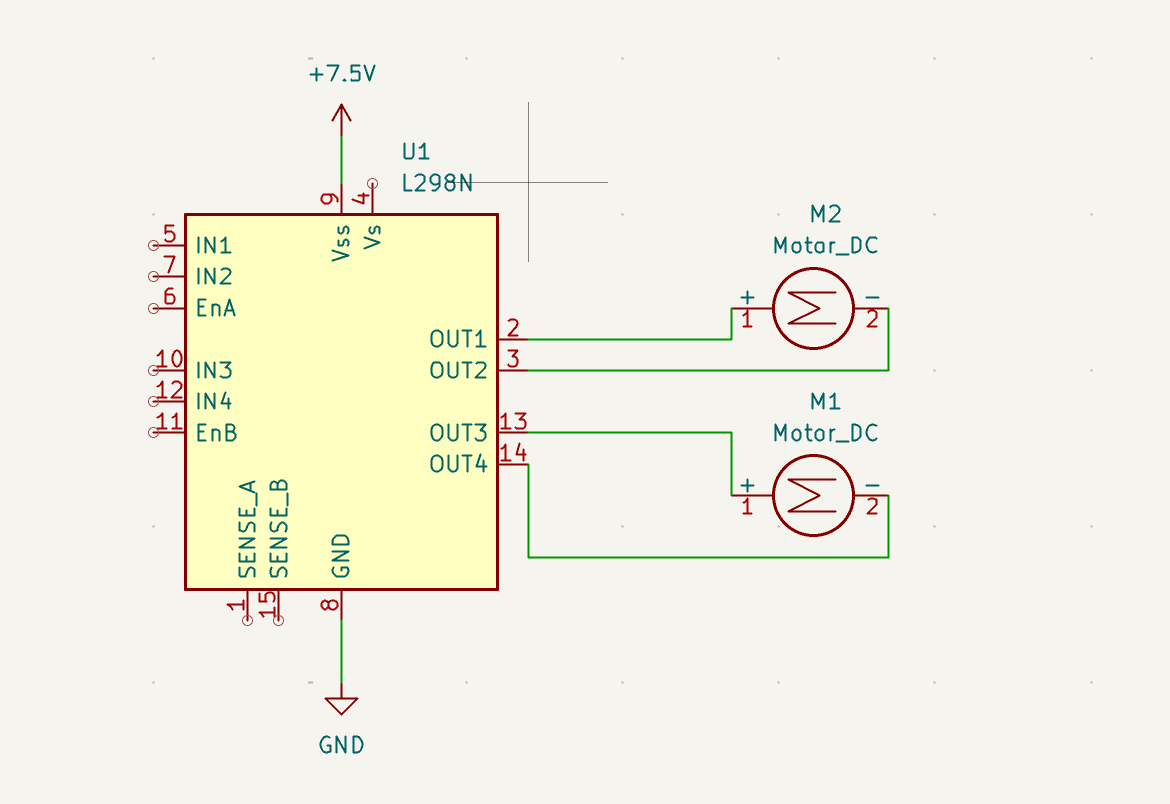
\includegraphics[width=\linewidth]{images/diagram/tt_motor_l298.png}
    \caption{Diagram of connections between L289N with 2 6V TT gear motors}
    \label{fig:l298n_2_motors}
\end{figure}

\vspace{1em}

\par
Two TT motor consume of total 6V due to the parallel wiring method through L298N, this motor driver 
allow power input in range from 5V to 12V, the maximum current <=2A, which are enough for two gear motors with total 
maximum current consume are ~600mA. All calculation follow the Ohm's law, parallel connected module share constant voltage 
with cumulative currents. 

\textbf{Ohm's law}
\[
V = IR
\]

\textbf{Total current of parallel gear arrangement}
\[
I_{\text{total}} = I_1 + I_2 + \cdots + I_n 
\]


\begin{figure}[H]
    \centering
    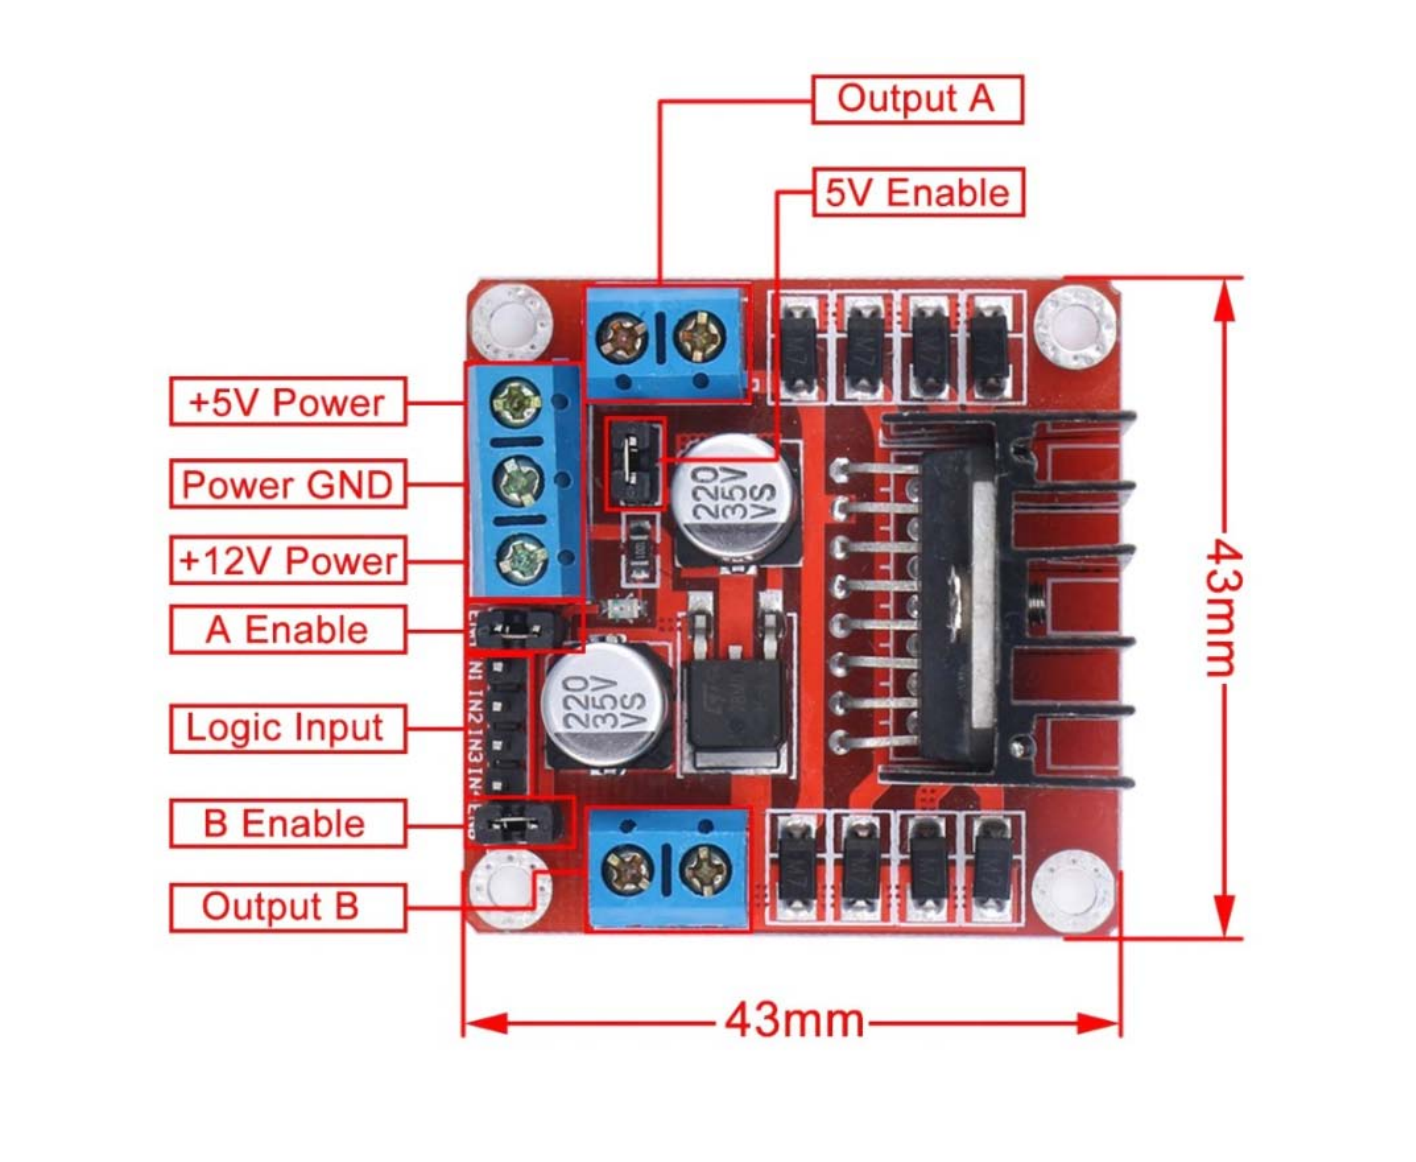
\includegraphics[width=0.8\linewidth]{images/electrical_schematics/L298N_image.png}
    \caption{L298N H-bridge DC motor driver }
    \label{fig:l298n_image}
\end{figure}


\begin{figure}[H]
    \centering
    
\includegraphics[width=0.9\linewidth]{/Users/nguyenthanhvinh/Documents/Papers/reference/final_maven_01_thesis/images/electrical_schematics/L298N.png}
    \caption{Schematic Diagram of L298N H-bridge DC motor driver }
    \label{fig:l298_schematic}
\end{figure}



\begin{figure}[H]
    \centering
    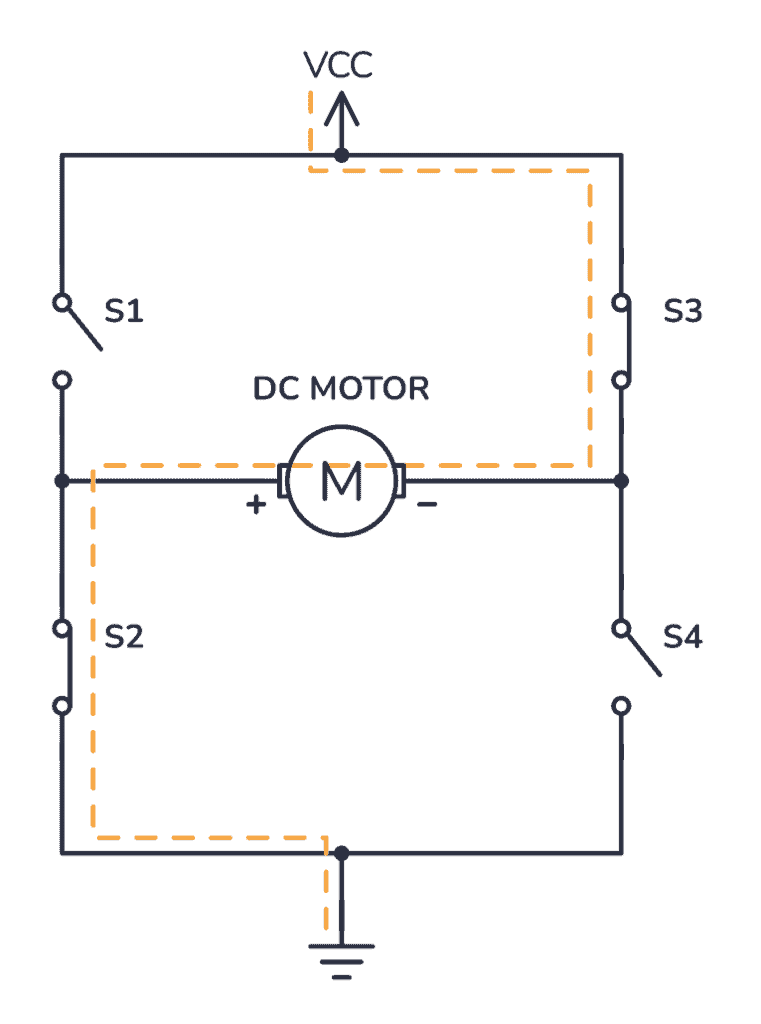
\includegraphics[width=0.5\linewidth]{images/electrical_schematics/h_bridge.png}
    \caption{Schematic Diagram of L298N H-bridge DC motor driver }
    \label{fig:h_bridge_image}
\end{figure}




L298N has a structure called an H-bridge, which allows it to have a total of 4 cases of current direction to control DC motors. 
In Figure~\ref{fig:h_bridge}, we can see an example of a single motor in an H-bridge circuit. 
When \verb|S3| and \verb|S1| are closed, it allows DC current to run through the motor, making it spin counterclockwise. 
On the other hand, if \verb|S1| and \verb|S4| are closed while \verb|S3| and \verb|S2| are open, DC current will run through and make the motor spin in the clockwise direction. L298N has two H-bridge circuits, which in theory can control more than 2 DC motors, as long as the current limit is not exceeded.

\vspace{1.5em}
\par
During the development process, we tested with 1 and 2 DC motors on each bridge and concluded that the L298N can handle 4 DC motors with a total current of approximately 1.2A. 
However, the movement capability will be similar to using 2 motors since the L298N only has 2 H-bridges.
 For better control and manipulation, we decided to switch to a 4-channel motor driver module.

\subsection{Control Protocol}

MAVEN-01 was designed to be teleoperated, so it needs a control board that has some kind of wireless send-and-receive mechanism.
Most of the time, radio signal is the first choice because of its wide range, stable connection, and relatively low power consumption.
However, complete radio control requires a full set including a remote control, transmitter, receiver, etc., which increases the overall cost significantly.

\vspace{1.5em}
In our project, we choose Wi-Fi as the main method to control the rover, not only for control but also to receive data from sensors attached to the rover. 
Because MAVEN-01 is designed for research purposes, Wi-Fi is a better choice. We only need a Wi-Fi built-in microcontroller board such as ESP32 or ESP8266. 
Sensor data are usually complex, so they require a high-bandwidth and low-latency signal to transmit. In this case, Wi-Fi performs better than radio, but the trade-off is higher latency 
and power consumption due to the higher frequency compare to normal radio signal.

\vspace{1.5em}


\subsection{Control Unit: WEMOS D1 R32 (ESP32 based)}
ESP32 is a microcontroller board with built-in WiFi and Bluetooth that we chose as the main control unit.
With its integrated WiFi module, it enables wireless control and sensor data transmission.
Compared to other boards such as Arduino UNO R4 or ESP8266, ESP32 offers faster processing speed and more GPIO pins, 
allowing more sensors to be connected. It is also affordable.

\vspace{1.5em}\par
\textbf{Board Comparison}

\begin{table}[h]
\centering
\begin{tabular}{|l|c|c|c|}
\hline
\textbf{Feature} & \textbf{ESP32} & \textbf{Pico W} & \textbf{UNO R4} \\
\hline
CPU & Dual-core 240 MHz & Dual-core 133 MHz & 48 MHz Cortex-M4 \\
\hline
RAM & 520 KB & 264 KB & 32 KB \\
\hline
Flash & 4 MB & 2 MB & 256 KB \\
\hline
WiFi & Yes & Yes & Yes \\
\hline
Bluetooth & Yes & No & No \\
\hline
GPIO & $\sim$30 & 26 & 14 \\
\hline
RTOS & Yes (FreeRTOS) & No & No \\
\hline
Power & Medium & Low & Low \\
\hline
Price (VND) & $\sim$120k & $\sim$180k & $\sim$700k--1M \\
\hline
\end{tabular}
\caption{Comparison of ESP32, Pico W, and Arduino UNO R4 WiFi}
\end{table}

ESP32 has many variants suitable for specific tasks. 
It also supports camera modules such as OV2640 or OV5640 for video streaming, making it suitable as an FPV camera for the rover.
In MAVEN-01, we used an Arduino-based ESP32 board called \href{https://handsontec.com/dataspecs/module/ESP/WeMos%20D1%20R32.pdf}{WEMOS D1 R32}. 
This board uses the same dual-core processor and features as the standard ESP32 from \href{https://www.espressif.com/}{Espressif}, 
but is easier to use due to its Arduino-like form factor.


\begin{figure}[H]
    \centering
    \includegraphics[width=\linewidth, page= 6]{images/electrical/d1_r32.png}
    \caption{Wemos D1 R32 pins maps, more information about detailed pinout description in \href{https://documentation.espressif.com/esp32-wroom-32d_esp32-wroom-32u_datasheet_en.pdf}{here}}
    \label{fig:chasis_1_engine_blueprint}
\end{figure}



\newpage
\subsection{Temperature ana humidity sensor: DHT11}
\par
\textbf{Overview}
\vspace{1em}

DHT11 Temperature \& Humidity Sensor features a temperature \& humidity sensor
complex with a calibrated digital signal output. By using the exclusive digital-signal-acquisition
technique and temperature \& humidity sensing technology, it ensures high reliability and
excellent long-term stability. This sensor includes a resistive-type humidity measurement
component and an NTC temperature measurement component, and connects to a highperformance 8-bit microcontroller, offering excellent quality, fast response, anti-interference
ability and cost-effectiveness.

\vspace{1em}
Each DHT11 element is strictly calibrated in the laboratory that is extremely accurate on
humidity calibration. The calibration coefficients are stored as programmes in the OTP memory,
which are used by the sensor’s internal signal detecting process. The single-wire serial interface
makes system integration quick and easy. Its small size, low power consumption and up-to-20
meter signal transmission making it the best choice for various applications, including those
most demanding ones. The component is 4-pin single row pin package. It is convenient to
connect and special packages can be provided according to users’ request.

\begin{figure}[H]
    \centering
    \includegraphics[width=\linewidth, page= 6]{images/information/dht_11/dht11_specification.png}
    \caption{DHT11 detailed specifications table, more information in \href{https://www.mouser.com/datasheet/2/758/DHT11-Technical-Data-Sheet-Translated-Version-1143054.pdf?srsltid=AfmBOoo4KPsepnO3XUCcgH6oYdE1Du44-sTxlVKOcYUqFeMKRha0P2Xu}{here} }
    \label{fig:dht11_spec_table}
\end{figure}

\par
\textbf{Power and pins}
\par
DHT11’s power supply is 3-5.5V DC. When power is supplied to the sensor, do not send any
instruction to the sensor in within one second in order to pass the unstable status. One
capacitor valued 100nF can be added between VDD and GND for power filtering.

\newpage

\textbf{ Communication Process: Serial Interface (Single-Wire Two-Way)}
\par
Single-bus data format is used for communication and synchronization between MCU and
DHT11 sensor. One communication process is about 4ms.
Data consists of decimal and integral parts. A complete data transmission is 40bit, and the
sensor sends higher data bit first.
Data format: 8bit integral RH data + 8bit decimal RH data + 8bit integral T data + 8bit decimal T
data + 8bit check sum. If the data transmission is right, the check-sum should be the last 8bit of
"8bit integral RH data + 8bit decimal RH data + 8bit integral T data + 8bit decimal T data".

\vspace{1.5em}

\textbf{Overall Communication Process}
\par

When MCU sends a start signal, DHT11 changes from the low-power-consumption mode to the
running-mode, waiting for MCU completing the start signal. Once it is completed, DHT11 sends a
response signal of 40-bit data that include the relative humidity and temperature information to
MCU. Users can choose to collect (read) some data. Without the start signal from MCU, DHT11
will not give the response signal to MCU. Once data is collected, DHT11 will change to the lowpower-consumption 
mode until it receives a start signal from MCU again.

\begin{figure}[H]
    \centering
    \includegraphics[width=\linewidth, page= 6]{images/information/dht_11/dht11_communciation.png}
    \caption{Detailed DHT 11 communication signal figure with MCU }
    \label{fig:dht11_comms_mcu}
\end{figure}


\vspace{1.5em}
Data Single-bus free status is at high voltage level. When the communication between MCU and
DHT11 begins, the programme of MCU will set Data Single-bus voltage level from high to low
and this process must take at least 18ms to ensure DHT’s detection of MCU's signal, then MCU
will pull up voltage and wait 20-40µs for DHT’s response.

\vspace{1.5em}
\textbf{MCU send 'wake up' signal to DHT11}
\begin{figure}[H]
    \centering
    \includegraphics[width=\linewidth, page= 6]{images/information/dht_11/dht11_signout.png}
    \caption{MCU Sends out Start Signal \& DHT Responses}
    \label{fig:mcu_start_dht11}
\end{figure}

\newpage
\textbf{DHT11 'waves back' to the MCU}

Once DHT detects the start signal, it will send out a low-voltage-level response signal, which
lasts 80µs. Then the programme of DHT sets Data Single-bus voltage level from low to high and
keeps it for 80µs for DHT’s preparation for sending data.
When DATA Single-Bus is at the low voltage level, this means that DHT is sending the response
signal. Once DHT sent out the response signal, it pulls up voltage and keeps it for 80µs and
prepares for data transmission.
When DHT is sending data to MCU, every bit of data begins with the 50µs low-voltage-level and
the length of the following high-voltage-level signal determines whether data bit is "0" or "1"
,see Figures ~\ref{fig:dht11_data_0} and ~\ref{fig:dht11_data_1}.


\begin{figure}[H]
    \centering
    \includegraphics[width=\linewidth, page= 6]{images/information/dht_11/dht11_data_0.png}
    \caption{ Data "0" Indication}
    \label{fig:dht11_data_0}
\end{figure}


\begin{figure}[H]
    \centering
    \includegraphics[width=\linewidth, page= 6]{images/information/dht_11/dht11_data_1.png}
    \caption{Data "1" Indication}
    \label{fig:dht11_data_1}
\end{figure}

\newpage
\textbf{Electrical Characteristics}
\begin{figure}[H]
    \centering
    \includegraphics[width=\linewidth, page= 6]{images/information/dht_11/dht11_electric_table.png}
    \caption{DHT11's electrical characteristics table}
    \label{fig:dht11_electrical_characteristic_table}
\end{figure}


\subsection{Distance measurement sensors: HC-SR04}
Ultrasonic is an excellent way of figuring out what’s in the immediate vicinity of your Arduino. The basics
of using ultrasound are like this: you shoot out a sound, wait to hear it echo back, and if you have your
timing right, you’ll know if anything is out there and how far away it is. This is called echolocation and it’s
how bats and dolphins find objects in the dark and underwater, though they use lower frequencies than you
can use with your Arduino.Figure-1 show the working principal of ultrasonic ranging concept.

\vspace{1.5em}
\href{https://www.handsontec.com/dataspecs/HC-SR04-Ultrasonic.pdf}{HC-SR04} Ultrasonic Sensor is a very affordable proximity/distance sensor that has been used mainly for
object avoidance in various robotics projects. It has also been used in turret applications, water level sensing,
and even as a parking sensor.
This module is the second generation of the popular HC-SR04 Low Cost Ultrasonic Sensor. Unlike the first
generation HC-SR04 that can only operate between 4.8V~5V DC, the improved version has wider input voltage
range, allow it to work with controller operates on 3.3V.HC-SR04 ultrasonic sensor provides a very low-cost
and easy method of distance measurement. It measures distance using sonar, an ultrasonic (well above
human hearing) pulse (~40KHz) is transmitted from the unit and distance-to-target is determined by
measuring the time required for the echo return. This sensor offers excellent range accuracy and stable
readings in an easy-to-use package. An on board 2.54mm pitch pin header allows the sensor to be plugged
into a solderless breadboard for easy prototyping


\textbf{Module specification}


\begin{figure}[H]
    \centering
    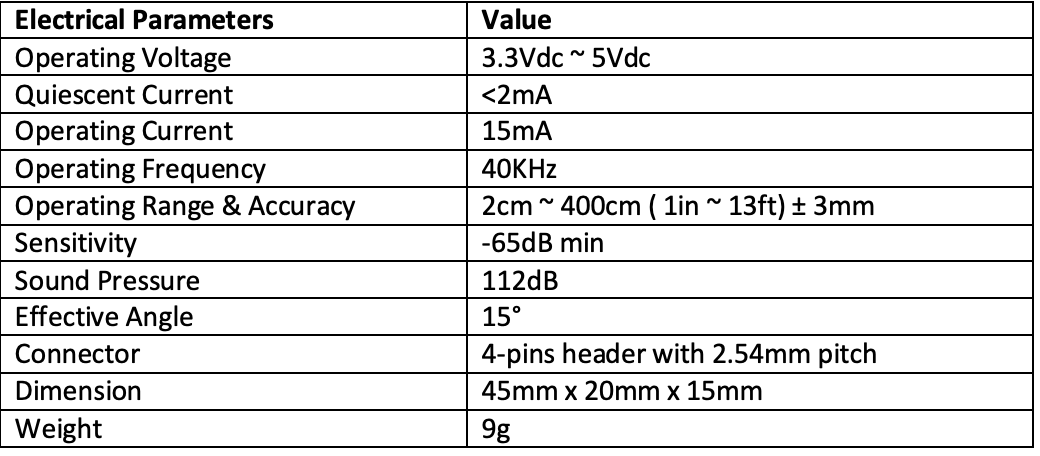
\includegraphics[width=\linewidth]{images/electrical/hc_sr04.png}
    \caption{HC-SR04 specifications table }
    \label{fig:hcSr04_specifications}
\end{figure}


The timing diagram, Figure~\ref{fig:hcSr04_schematic_timing}  is shown below. You only need to supply a short 10uS pulse to “Trigger Input”
pin to start the ranging. The module will send out 8-cycles burst of ultrasound at 40KHz and raise its “Echo” 
6 pin, refer to Figure~\ref{fig:hcSr04_schematic_mcu}. The echo is a distance object that is pulse width and the range in proportion. You can
calculate the range through the time interval between sending trigger signal and receiving echo signal.
Formula: µS / 58 = centimeters or µS / 148 =inch
or: the range = high level time * sound velocity (340m/s) / 2; 

\begin{figure}[H]
    \centering
    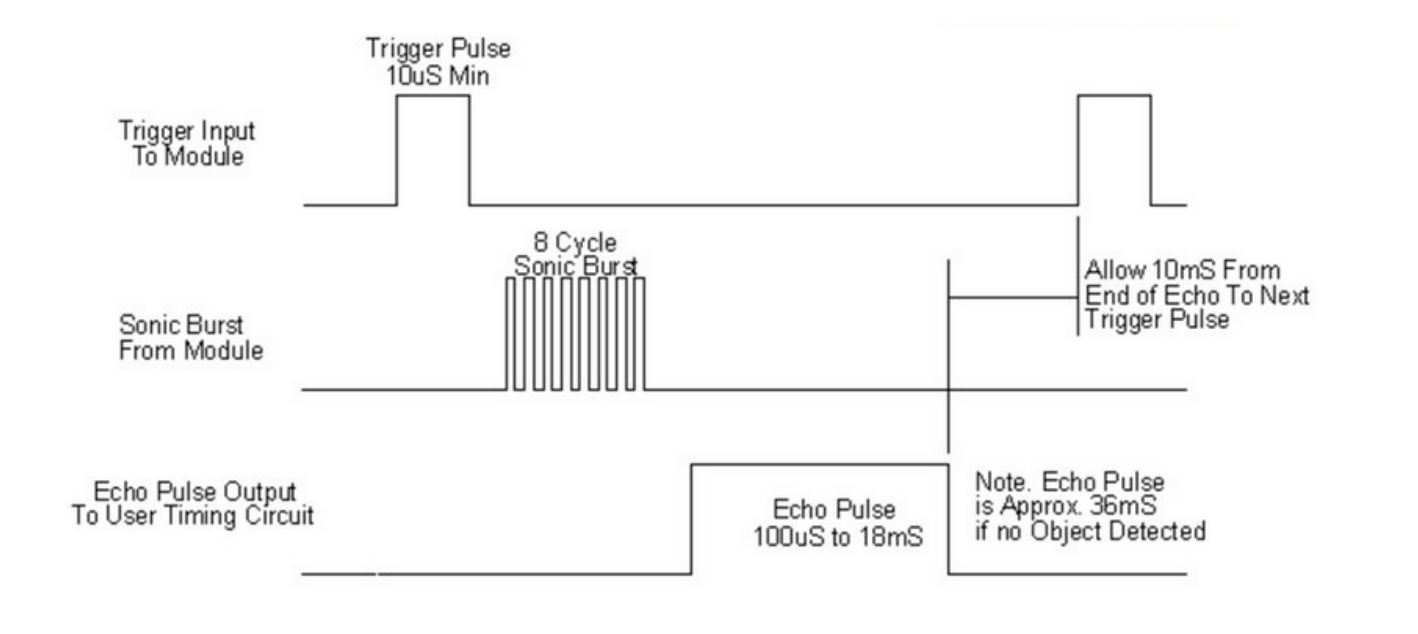
\includegraphics[width=\linewidth]{images/electrical_schematics/hcsr04_timing.png}
    \caption{HC-SR04 timing schematic diagram}
    \label{fig:hcSr04_schematic_timing}
\end{figure}

\begin{figure}[H]
    \centering
    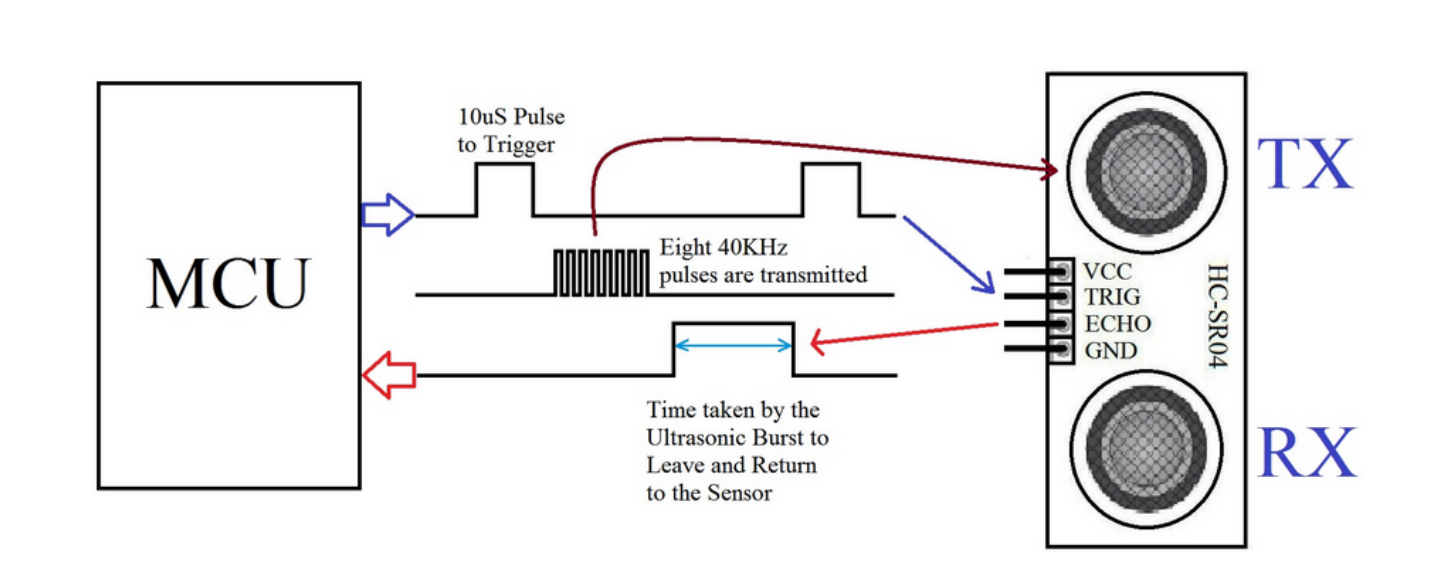
\includegraphics[width=\linewidth]{images/electrical_schematics/hcsr04_mcu.png}
    \caption{HC-SR04 timing schematic diagram}
    \label{fig:hcSr04_schematic_mcu}
\end{figure}


\subsection{IMU sensor: MPU 9250}
\par
The MPU-9250 is a compact 9-axis motion tracking sensor developed by \href{https://invensense.tdk.com/en-us}{TDK InvenSense}. 
It integrates three sensing components into a single chip:\verb|accelerometer, gyroscope, magnetometer|.
This module is more superior than older IMU sensor generation like MPU 6050. By integrated 9 axis for 3 sensors in 1 module, it helps
simplify electrical system while provide the same functions that requires multiple modules. This combination enables full 9 degrees of freedom 
(9-DoF) motion tracking, making the MPU-9250 suitable for applications requiring orientation, motion detection, and navigation.


\begin{figure}[H]
    \centering
    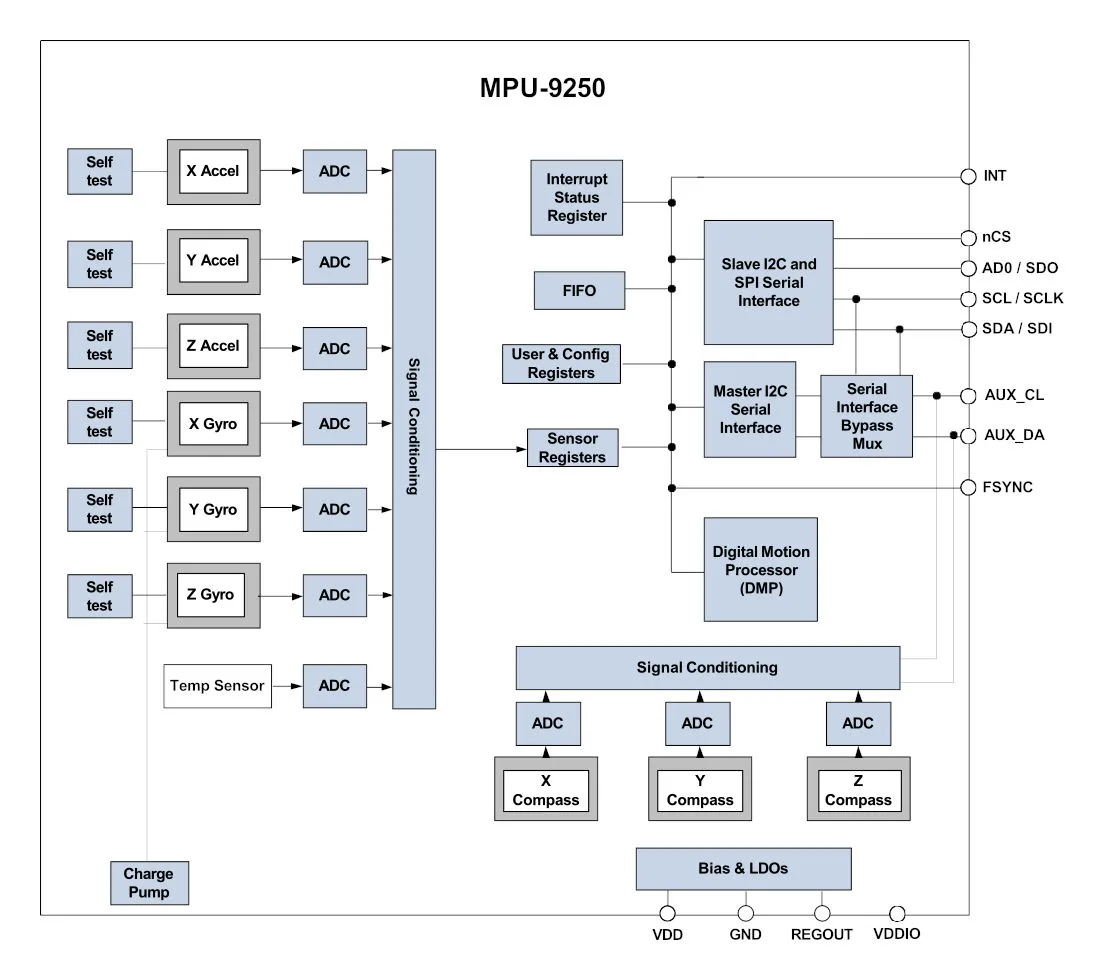
\includegraphics[width=\linewidth]{images/electrical_schematics/mpu9250-block-diagram.png}
    \caption{MPU-9250 block diagram, more information can be found in this \href{https://cdn.sparkfun.com/assets/learn_tutorials/5/5/0/MPU9250REV1.0.pdf}{datasheet}, announced by TDK InvenSense}
    \label{fig:mpu9250_diagram}
\end{figure}


\textbf{Overview}
\par
In this part, we not dive into detailed and technical specification, we only focus 3 main general 
functions are: \textbf{gyroscope, accelerometer and magnetometer}

\vspace{1.5em}
\par
The MPU-9250 consists of three independent vibratory MEMS rate gyroscopes, which detect rotation about
the X-, Y-, and Z- Axes. When the gyros are rotated about any of the sense axes, the Coriolis Effect causes
a vibration that is detected by a capacitive pickoff. The resulting signal is amplified, demodulated, and filtered
to produce a voltage that is proportional to the angular rate. This voltage is digitized using individual on-chip
16-bit Analog-to-Digital Converters (ADCs) to sample each axis. The full-scale range of the gyro sensors
may be digitally programmed to ±250, ±500, ±1000, or ±2000 degrees per second (dps). The ADC sample
rate is programmable from 8,000 samples per second, down to 3.9 samples per second, and user-selectable
low-pass filters enable a wide range of cut-off frequencies.

\vspace{1.5em}
\par
The MPU-9250’s 3-Axis accelerometer uses separate proof masses for each axis. Acceleration along a
particular axis induces displacement on the corresponding proof mass, and capacitive sensors detect the
displacement differentially. The MPU-9250’s architecture reduces the accelerometers’ susceptibility to
fabrication variations as well as to thermal drift. When the device is placed on a flat surface, it will measure
0g on the X- and Y-axes and +1g on the Z-axis. The accelerometers’ scale factor is calibrated at the factory
and is nominally independent of supply voltage. Each sensor has a dedicated sigma-delta ADC for providing
digital outputs. The full scale range of the digital output can be adjusted to ±2g, ±4g, ±8g, or ±16g


\vspace{1.5em}
\par 
The 3-axis magnetometer uses highly sensitive Hall sensor technology. The magnetometer portion of the IC
incorporates magnetic sensors for detecting terrestrial magnetism in the X-, Y-, and Z- Axes, a sensor driving
circuit, a signal amplifier chain, and an arithmetic circuit for processing the signal from each sensor. Each
ADC has a 16-bit resolution and a full scale range of ±4800 µT.


\subsection{Buck converter: LM2596}

Sensors used in MAVEN-01 like MPU, DHT11 work stable at 3.3V, but the power supply provide 6V, which mean if we connect it
directly to sensors, sensors will be damaged, so we need \href{https://www.ti.com/lit/ds/symlink/lm2596.pdf}{LM2596} 
to lower the voltage.


\begin{figure}[H]
    \centering
    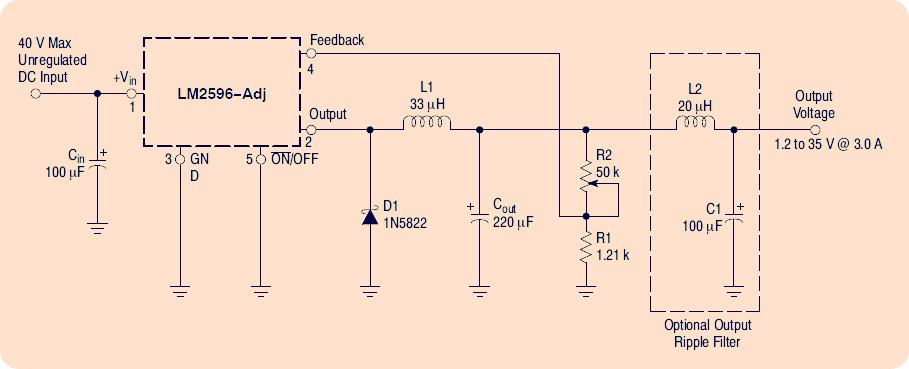
\includegraphics[width=\linewidth]{images/diagram/LM2596.png}
    \caption{LM2596 block diagram, more information can be found in this \href{https://www.alldatasheet.com/datasheet-pdf/view/543770/TI1/LM2596.html}{datasheet}, announced by Texas Instruments}
    \label{fig:lm2596_diagram}
\end{figure}

\begin{figure}[H]
    \centering
    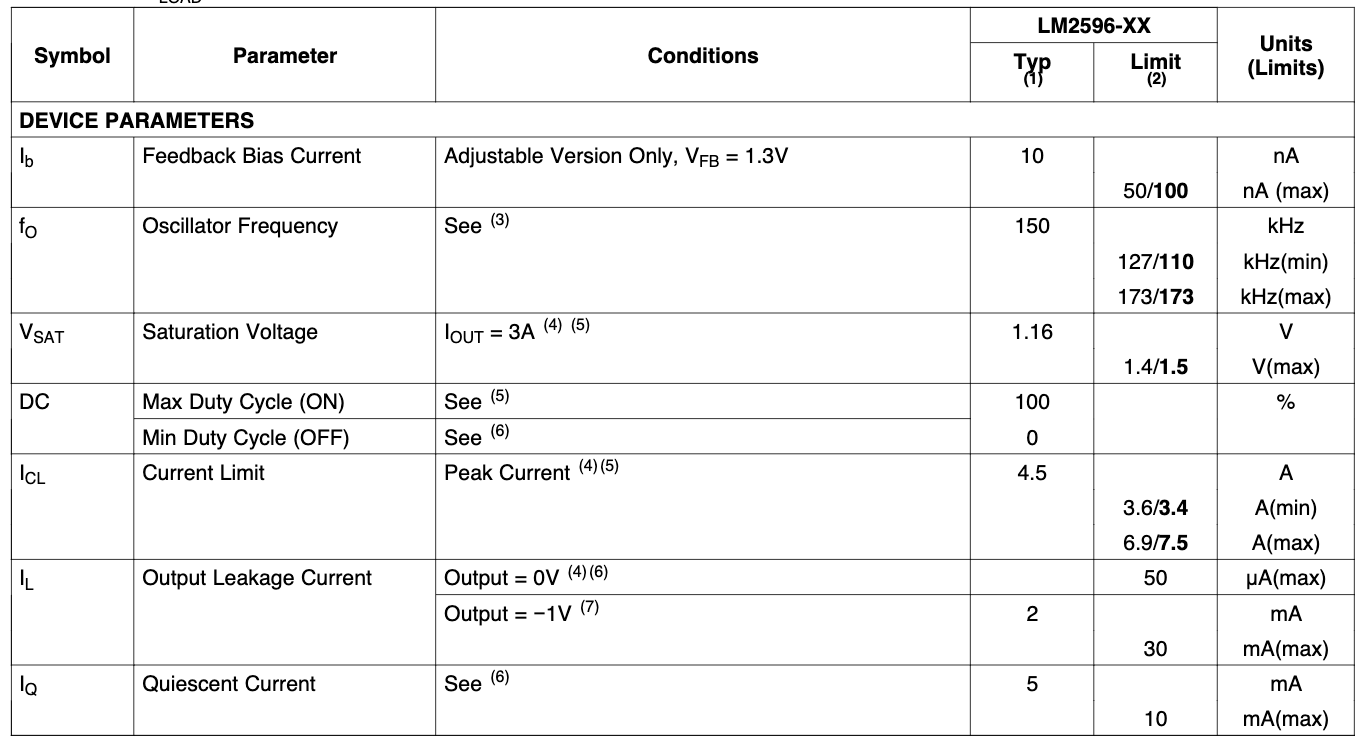
\includegraphics[width=\linewidth]{images/information/lm2596_spec.png}
    \caption{LM2596 specifications table}
    \label{fig:lm2596_tables}
\end{figure}



\subsection{Power source}
In Diagram~\ref{fig:maven_01_system_architecture}, MAVEN-01 was designed with three separate power sources. 
This design lays the groundwork for stable operation and minimizes chain-reaction failures. For instance, if any part of MAVEN-01 fails 
for any reason, we can easily identify the cause and immediately disconnect the faulty part from the system without shutting down 
the entire system.

\vspace{1em}
\par
For the microcontroller board, we use a 9V box battery since the Wemos D1 R32 board supports a voltage range 
from 9V to 12V. For all sensors, we use four AA batteries with a total output of 6V, but we use an LM2596 buck converter to reduce the voltage
to 3.3V in order to avoid damaging the sensors. For the motor power supply, we use two 18650 3.7V batteries with a high current rating of 13A and a total capacity of 5200mAh,
which is more than enough for 6--8V TT gear motors. However, when MAVEN-01 is upgraded, we will not need to replace the entire power supply system, making it more cost-efficient.
























\newpage
\section{Software Design}
\subsection{Control and Monitoring system} 
\label{sec:monitoring}

For the first version of control and monitoring GUI, we will using QT framework 
with Python. Main features of the system is to monitor sensors data receive from MAVEN-01, velocity 
battery level and many other features. This system will information intuitively about the condition
of environments surround the rover which is the main target of MAVEN-01.

\vspace{1.5 em }
\href{https://www.qt.io/development/qt-framework}{QT framework} is flexible framework for making desktop application, compatible with both Python and C++,
more specific, MMS was using Pyside6, a library that allow users use QT APIS through Python. 

 \begin{figure}[H]
    \centering
    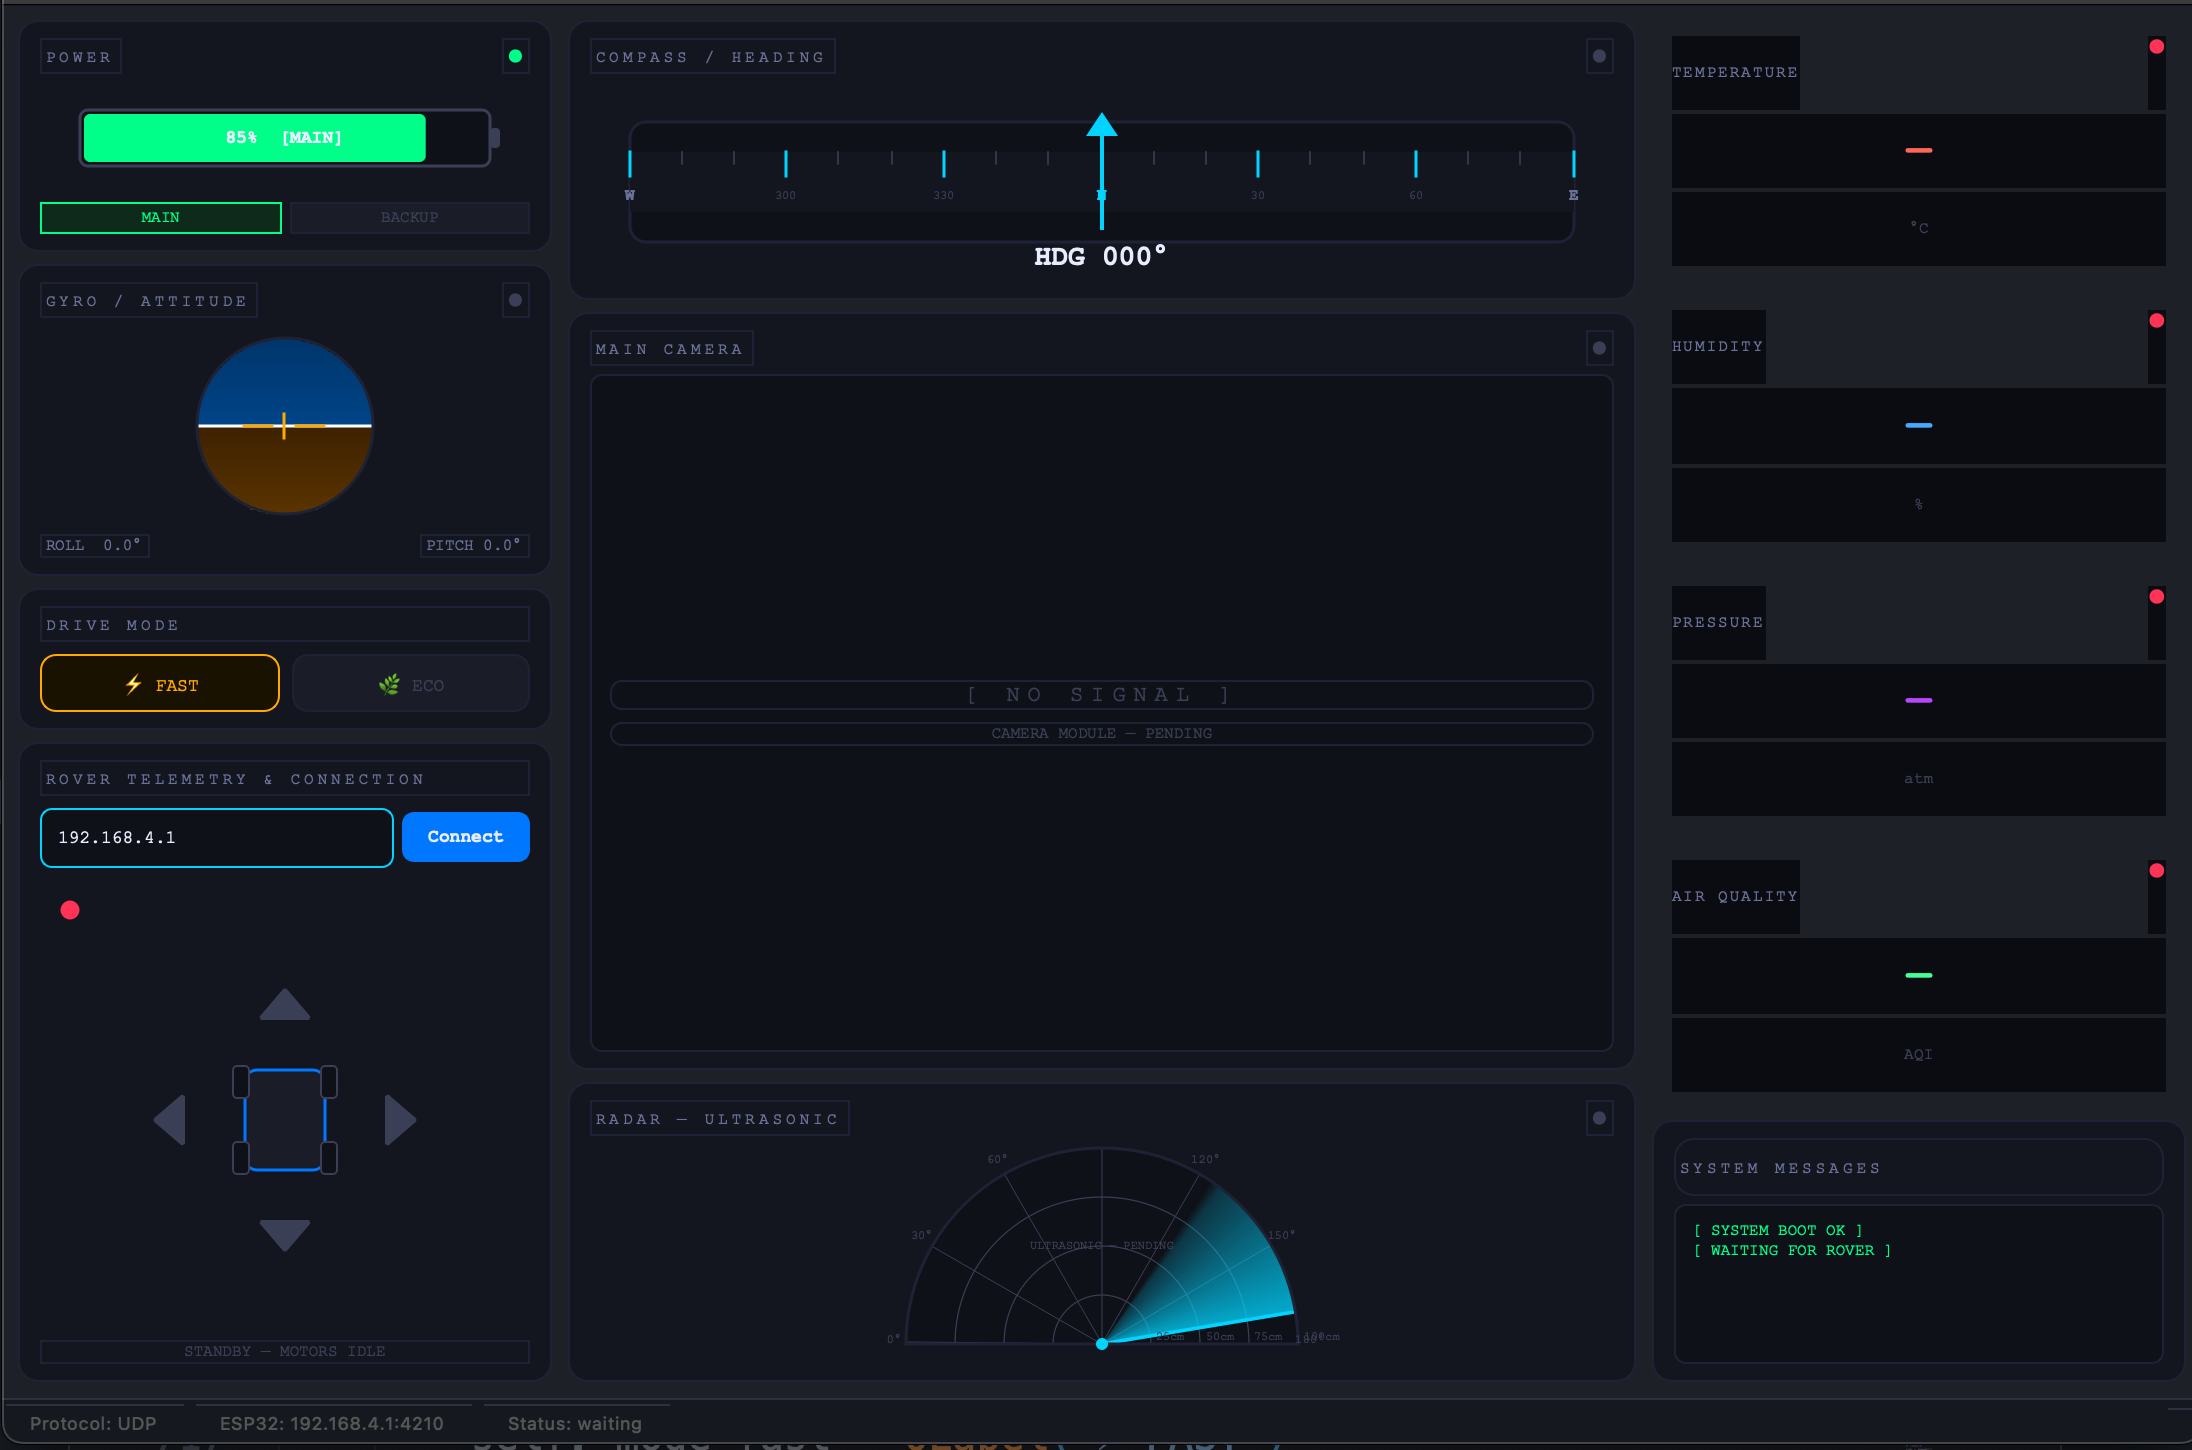
\includegraphics[width=\linewidth]{images/demo/MMS_1st_vers.png}
    \caption{Main user interface of MMS first version }
    \label{fig:mms_ui_demo_1}
\end{figure}

\textbf{Control Signal}
\par
To display the sensor data, the control system defines different ports for sending and receiving messages. For the MMS, there are two signal messages used for control. 
The first is a checking message to confirm that the controller board is connected to the control station. After that, the control signals are transmitted in the form of key-value pairs, 
such as {control: left} and {control: right}.
 

\vspace{0.5em}
\par
Two UDP sockets are created: a transmission socket for sending commands and a reception socket for listening to incoming packets. 
To prevent the graphical user interface (GUI) from freezing during network operations, a dedicated background thread continuously monitors incoming UDP messages. The \verb|start()| method initializes 
the receiver socket and launches the listening thread, while the \verb|stop()| method safely terminates communication and closes all sockets.

\vspace{0.5em}

\par
The \verb|send_command()| function packages motor control instructions, including the movement direction and speed, into JSON format before transmitting them to the ESP32. This structured data format 
simplifies message parsing and enhances communication reliability. The \verb|update_esp_ip()| method allows the target ESP32 IP address to be modified dynamically during runtime, providing flexibility when network configurations change.
The \verb|_recv_loop()| method operates continuously in a separate thread to receive and process incoming UDP packets from the ESP32. Upon receiving data, the JSON.

\subsection{Sensors data transportation protocol: Wifi + UDP}
\par
To connect from MMS to the Rover, we use Wifi \& UDP based protocol,
a lightweight, low latency network protocol designed for low-bandwidth, unreliable networks and 
resource-constrained IoT devices. Maven-01’s main goal is to go to hazardous places and collect environmental information such as pressure, 
temperature, and humidity. Even though the 2.4 GHz Wi-Fi bandwidth is quite large,it is not very stable when the rover is covered by obstacles.
Therefore, we still need UDP for low-latency and robust data transmission.

\par

The WEMOS D1 R32 module creates a local 2.4 GHz Wi-Fi network to establish wireless communication between the rover and the MMS control system. 
Through this connection, control commands and telemetry data are transmitted simultaneously using UDP packets formatted in JSON (for e.g "temperature": 20).
\vspace{1.5 em}

\begin{figure}[H]
    \centering
    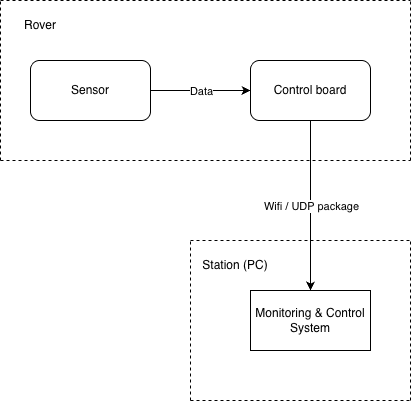
\includegraphics[width=0.7\linewidth]{images/diagram/sensors_data_udp.png}
    \caption{Sensor data transportation workflow diagram}
    \label{fig:udp_sensor_diagram}
\end{figure}


\subsection{Control Protocol: 2.4 GHz Bandwidth Wifi}

\vspace{1em}
\par 
In the previous section, Wifi \& UDP based protocol was discussed as the main protocol used for data transportation, the control communication protocol 
used in the MMS for MAVEN-01 was the same to it. If we look deeper into rover systems and many other UGVs (Unmanned Ground Vehicles), low-latency control
plays a crucial role in overall performance. In MAVEN-01, Wi-Fi serves as the main communication protocol between the rover and the monitoring system, while 
UDP acts as the constant signal transmission protocol.

\vspace{1.5em}
Unlike TCP, which uses a \textit{``make sure the packet is received by the receiver''} mechanism before sending the next packet, UDP removes this confirmation process and continuously sends signals without waiting for acknowledgment. This significantly reduces latency. For this reason, time-critical systems often prefer UDP over other communication protocols.

\vspace{1em}
However, one problem we had to deal with was that the control signals and sensor data might conflict with each other during transmission. To avoid this issue, we set the sending frequency of the control signals higher than the sensor data transmission frequency. This works similarly to two cars not driving parallel to each other on the same road, helping to reduce communication interference and improve the response speed of the rover control system.
\begin{figure}[H]
    \centering
    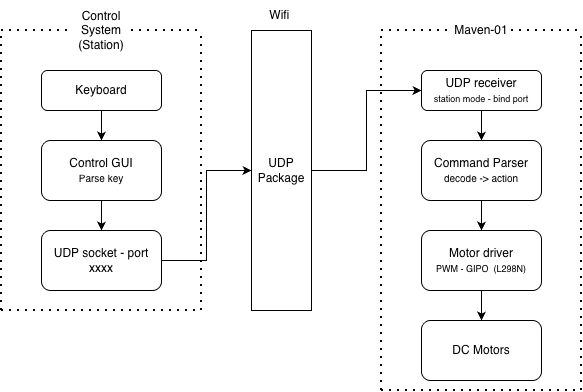
\includegraphics[width=\linewidth]{images/diagram/protocol/control.drawio_new.png}
    \caption{UDP control workflow diagram}
    \label{fig:udp_control_diagram}
\end{figure}


Figure~\ref{fig:udp_control_diagram} illustrates the UDP-based control workflow used in MAVEN-01. The control process begins at the monitoring station, where keyboard inputs are interpreted by the control GUI and transmitted through a UDP socket over a Wi-Fi connection. On the rover side, 
the UDP receiver obtains the transmitted packets and forwards them to the command parser for decoding.The decoded commands are then sent to the motor driver, which controls the DC motors through GPIO signal which is allowed workflow enables low-latency communication for real-time rover control.

\vspace{1em}
During the development and testing phase, MAVEN-01 experienced some issues with connection and signal transport latency. When the WEMOS D1 R32 broadcasts a Wi-Fi signal, by default,
if it does not receive a control signal sent from the control system, it automatically turns off the Wi-Fi module for a very short time to save energy. To solve this problem, we had to turn off the power-saving mode and allow the board to 
broadcast Wi-Fi continuously at all times. However, the trade-off is that the system becomes more power-hungry, so we need a stable and high-capacity power supply for MAVEN-01 to operate properly, which is already mentioned in Section 4.7.
\newpage
\input{sections/etics}
\newpage
\input{sections/contribs}
\newpage
\input{sections/results}
\newpage
\input{sections/discussion}
\newpage
\section{Testing}
In this section, we will test MAVEN-01 and capture the results to see how well it operates through
different types of terrain. Furthermore, the electrical system will also be evaluated in terms of battery usage time and operation. 
Sensor data will be checked to see how well the sensors capture data from the environment and how accurate the data are. Lastly, 
we will carry out the maintenance process to test how easy MAVEN-01 is to maintain, replace components, and recharge power.

\vspace{1em}
\par
The Wemos D1 R32 board can broadcast its own Wi-Fi, and we can connect to it using a password. During testing, the sensor data sent
to the control system and displayed on the control system monitor was quite accurate based on two references: the weather app on iOS 
and a home temperature and humidity meter.
\par
\vspace{0.5em}
Because of the 3-power-supply system, MAVEN-01 is very easy to maintain. 
If any components, such as sensors or the control board, run out of power or fail, 
we can easily change the battery corresponding to that component without shutting down the whole system. 
It is also not hard to find the source of failure due to the modular structure.

\vspace{0.5em}
\par
We only equipped one INA219 current sensor to measure the current and voltage 
of the power source that powers the controller board because of pin limitations, and 
the other components are less sensitive to power loss than the control board, which is the most important component 
in the rover. The working voltage range of the control board power source is between 9V and 7.4V. When the voltage reaches around 7.5V , we consider the 
battery to be almost depleted and in need of recharging or replacement to prevent electrical component failures.

\vspace{0.5em}
\par 
Most of the sensors run at 3.3V, so we power them with a separate power source. We use four 1.5V AA batteries through 
a buck converter to obtain a 3.3V output, and the batteries can also be replaced easily. For the motor power source, 18650 batteries with 
high power capacity are a good choice for longer operation time.

\section{Future Work}
\par
Since MAVEN-01 was created for research and educational purposes, it can be modified or 
improved in many different ways. I am a Data Science major student, so in the future I may implement 
reinforcement learning or an AI system on edge devices such as Orin or DGX, which could make MAVEN-01, or perhaps MAVEN-02 or MAVEN-03, operate autonomously 
without human control. This is a high-potential project that can provide me personally, as well as many other students 
or researchers, with experience and knowledge in the fields of robotics and AI.

\vspace{0.5em}
\par 
The materials can also be innovated and upgraded. For this very first version, I used PLA because it is cheap 
and easy to process, but its durability and flexibility cannot be compared to advanced filaments such as Nylon-CF or 
PETG-CF, etc. MAVEN has a modular structure, so it can be upgraded part by part, making it suitable for a tight budget.

\section{Acknowledge}

I would like to express my sincere gratitude to my supervisor PhD. Pham Xuan Tung for the guidance, support, and encouragement throughout this project. 
Your valuable knowledge and patience helped me complete this work successfully. I truly appreciate the time and effort you dedicated to helping me learn and improve.

\newpage
%\input{sections/Acknowledgments}
% ============================= References ============================
% \newpage
\printbibliography
\addcontentsline{toc}{section}{References}

% ============================ Appendices =============================
%\newpage
%\begin{appendices}

	%\input{appendices/appendices1}images/electrical_schematics/L298N.png
	%\clearpage
	
	%\input{appendices/appendices2}
	%\clearpage
	
%\end{appendices}

\end{document}
